\documentclass[sotsuron]{kuee}

\usepackage[dvipdfmx]{graphicx}
\usepackage{here}
\usepackage{amsmath}
\usepackage{bm}
\usepackage{multirow}


\title{DNAストレージにおけるナノポアシーケンサーの読み出し特性を考慮した誤り訂正手法}
\etitle{Error Correction Method Considering the Reading Characteristics of Nanopore Sequencers in DNA Storage}
\author{岩瀬 真太郎}
\eauthor{Shintaro Iwase}
\professor{佐藤 高史 教授}
% \course{京都大学大学院情報学研究科}
% \department{知能情報学専攻}
\date{令和8年2月10日}

%%% 本文
\begin{document}
\maketitle			% 表題を出力
\begin{eabstract}		% 英文要旨を出力
In today's information society, large amounts of digital data are generated 
every day, and the amount of data worldwide continues to grow explosively. 
DNA storage has emerged as a promising solution for long-term archival storage 
due to its high information density and durability. While nanopore sequencers 
offer advantages in reading long DNA sequences at high speeds, they suffer from 
lower accuracy compared to short-read sequencers, particularly with insertion 
and deletion errors. Although existing error-correcting codes have been proposed 
for DNA storage with capability to correct these errors, their decoding algorithms 
have not been optimized for the specific characteristics of nanopore sequencers.

This study aims to optimize existing error correction methods 
specifically for DNA storage systems using nanopore sequencers. The proposed 
method incorporates two key improvements: (1) optimization of reward and penalty 
parameters based on statistical transition matrices that model nanopore reading 
characteristics, and (2) integration of confidence scores from the basecaller's 
CTC (Connectionist Temporal Classification) output into the decoding process. 
Additionally, to address accuracy degradation with longer DNA sequences, we 
propose a segmentation-based encoding scheme that divides sequences into short 
segments with separators and reinitializes the hash function at segment boundaries.

Simulation results demonstrate that the proposed method improves 
both decoding efficiency and accuracy. The optimized decoding algorithm reduces 
heap search operations by 64-68\% and bit deletion rates by 76-83\% compared to 
the existing method. The segmentation scheme maintains stable decoding accuracy 
even for DNA sequences up to 15,000\,nt without significantly increasing computational 
complexity. 
% After Reed-Solomon outer decoding, the proposed method achieves a 77\% 
% error rate reduction at 0.75 coding rate compared to the existing method. These 
% results demonstrate that the proposed optimization makes nanopore sequencers more 
% practical and effective for DNA storage applications.

\end{eabstract}
\tableofcontents		% 目次を出力

\chapter{Introduction}
In today's information society, massive amounts of digital data are generated
every day, and the global volume of data continues to increase explosively.
According to a 2025 report, the total volume of digital data worldwide is
estimated to be 173.4 zettabytes, and is projected to reach 527.5 zettabytes
by 2029\cite{statista_worldwide_data_created}.
Among this vast amount of data, approximately 60\% is known to be cold data
that is accessed very infrequently\cite{dna_data_storage_alliance_2021_intro}.
Cold data includes information that must be retained for long periods to comply
with legal requirements and research data that may be analyzed in the future,
which makes deletion difficult.
Therefore, archival storage technologies that can store cold data for long
periods at low cost are strongly needed
\cite{reinsel2017dataage2025,dna_data_storage_alliance_2021_intro}.

% Introduction background DNA storage
In recent years, DNA storage has attracted attention as a next-generation
archival storage technology.
DNA storage is a technique in which digital data are encoded into sequences of
the four nucleotides adenine (A), cytosine (C), guanine (G), and thymine (T),
and then stored in synthetically generated DNA.
In addition to its high durability, which enables data preservation for
thousands of years under appropriate storage conditions, DNA storage is
expected to provide extremely high information density because a very large
amount of information can be stored per unit volume.
For these reasons, it is considered a promising new storage technology suitable
for preserving cold data
\cite{akash2024_applicable,Ceze2019,dna_data_storage_alliance_2021_intro}.

% DNA storage sequencer
In DNA storage, data are read by analyzing DNA base sequences using DNA
sequencers\cite{Ceze2019}.
DNA sequencers are broadly classified into short-read sequencers, which target
DNA with short lengths of several tens to several hundreds of bp
\footnote{Abbreviation of base pair. A unit representing sequence length in
double-stranded DNA. For single-stranded DNA, nucleotides are typically
represented by the unit nt.}
\cite{Simon2009}, and long-read sequencers, which target DNA with lengths from
several hundred to several tens of thousands of bp \cite{Amarasinghe2020}.
However, in many previous studies on DNA storage, short-read sequencers based
on SBS (Sequence By Synthesis)\cite{SBS} have mainly been used.
Although SBS provides highly accurate, massively parallel analysis of DNA
fragments, it has disadvantages such as a limited read length of only several
hundred bp at a time and relatively low sequencing speed\cite{SBS}.
In contrast, nanopore sequencers, one type of long-read sequencer, can analyze
very long DNA sequences of up to several hundred thousand bp at high speed,
and are therefore considered more practical for DNA storage readout
\cite{Amarasinghe2020}.
Accordingly, this study focuses on DNA storage systems that assume readout by
nanopore sequencers.

While nanopore sequencers can analyze long DNA sequences rapidly, their base
calling accuracy is known to be lower than that of SBS, especially due to the
high frequency of insertion and deletion errors
\cite{Amarasinghe2020,Dorey2024}.
Therefore, when nanopore sequencers are used in DNA storage, it is important to
investigate error-correcting codes that can handle insertion and deletion
errors in addition to substitution errors.

Previous work proposed error-correcting codes for DNA storage that satisfy
sequencing constraints, such as prohibiting consecutive identical bases
(homopolymers) and restricting GC content, while correcting substitution,
insertion, and deletion errors.
Through simulation and experiments using synthesized DNA, the study showed the
possibility of accurately recovering petabyte-scale data from base sequences
containing up to approximately 10\% errors\cite{HEDGES}.
However, the previous work assumed short-read sequencers for DNA storage
readout, and did not optimize the error-correcting code for the readout
characteristics of nanopore sequencers.
In addition, the previous method reported degraded decoding accuracy for longer
base sequences, and improving decoding accuracy for long sequences with
long-read sequencers such as nanopore sequencers remains a challenge.

In this study, we propose an error-correction method for DNA storage that
assumes readout with nanopore sequencers.
We optimize the decoding algorithm of existing error-correction methods by
incorporating the readout characteristics of nanopore sequencers to improve
both decoding efficiency and accuracy.
We also propose a method to suppress accuracy degradation when handling long
DNA sequences in the encoding process.
We evaluate the proposed method through simulations of the full pipeline, from
binary data encoding to nanopore-based readout and decoding.

\chapter{Encoding and Readout in DNA Storage}
\section{Overview of DNA Storage} \label{dna_storage}
DNA storage is a technology that encodes digital data into DNA base sequences
and stores data in synthetically generated DNA as a storage medium.
DNA storage performs data writing and readout through the following steps.
\begin{enumerate}
  \item Encoding\\
  First, binary data are encoded into DNA base sequences.
  During encoding, sequence constraints are imposed to suppress synthesis
  errors and maintain structural stability. Such constraints include
  prohibiting homopolymers and constraining GC content to a certain range
  \cite{Gervasio}.
  In addition to introducing redundancy for error correction during decoding,
  the encoded sequences must also be robust against errors generated during
  sequencing.
  \item Storage\\
  Synthetic DNA is generated based on the encoded base sequences. The synthesized
  DNA is commonly stored in a dry state to increase storage density and stability
  \cite{landsman2023the}.
  Under such conditions, long-term preservation over thousands of years is
  considered feasible \cite{Grass2015Robust}.
  \item Data readout\\
  To read data from stored DNA, DNA molecules are first extracted, and then
  their base sequences are analyzed using DNA sequencers such as SBS sequencers
  and nanopore sequencers, which are described in detail in
  Section~\ref{nanopore}.
  Three types of sequencing errors can occur:
  \begin{itemize}
    \item Substitution error: a read base differs from the original base.
    \item Insertion error: a base not present in the original sequence is read.
    \item Deletion error: a base present in the original sequence is not read.
  \end{itemize}
  The original binary data are reconstructed from sequences containing these
  errors by applying error correction.
\end{enumerate}

\section{HEDGES} \label{hedges}
HEDGES (Hash Encoded, Decoded by Greedy Exhaustive Search) is an
error-correction method that satisfies sequence constraints while correcting
substitution, insertion, and deletion errors \cite{HEDGES}.
\subsection{Encoding} \label{hedges_encoding}
In HEDGES, data are handled in packet units.
Each packet consists of 255 fixed-length DNA strands, and the base length of
each strand can be freely configured.
Encoding is performed in two stages: Reed-Solomon (RS) encoding, which converts
the input bitstream into an error-correctable bitstream, and HEDGES encoding,
which converts that bitstream into a base sequence with additional redundancy.
Figure~\ref{fig:hedges_encoding} shows an overview of HEDGES encoding.
\begin{figure}
    \begin{center}
        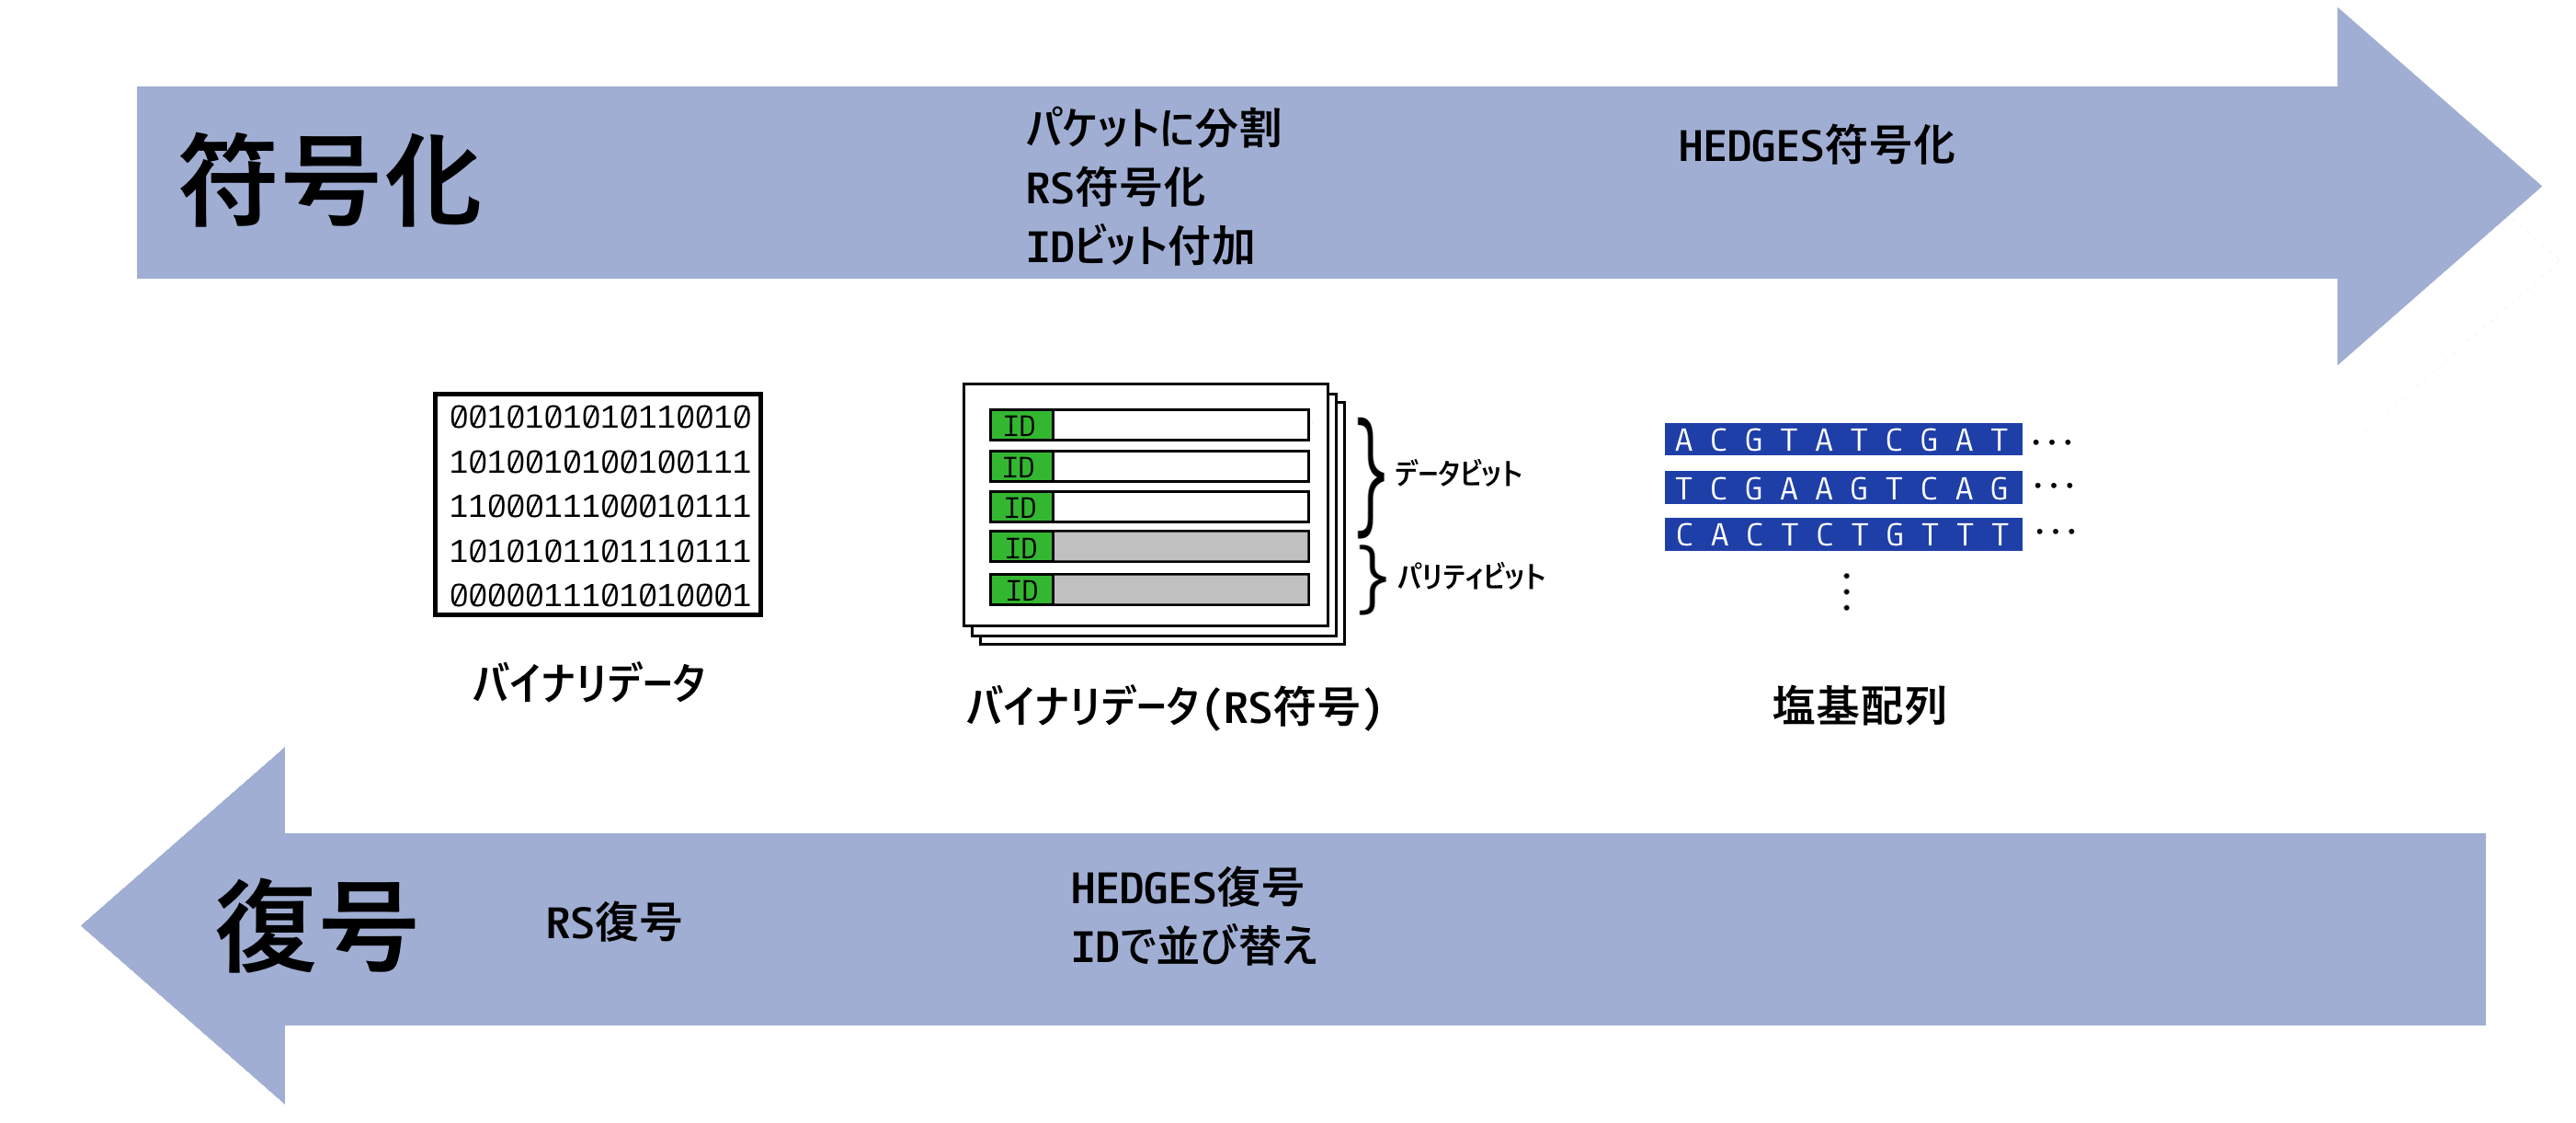
\includegraphics[width=150mm]{hedges.png}
        \caption{Overview of HEDGES encoding}\label{fig:hedges_encoding}
    \end{center}
\end{figure}
First, binary data are split into packets, and RS encoding is applied to each
packet to obtain one RS-encoded bitstream per packet.
This RS code is called the outer code and is responsible for final correction
of errors that remain after decoding from base sequence back to bitstream.
Next, HEDGES encoding, used as the inner code, is applied to the RS-encoded
bitstream to generate the base sequence.
One key feature of HEDGES is that the coding rate for bit-to-base conversion is
variable. By lowering the coding rate, additional redundancy can be introduced
to improve error-correction capability.

The specific HEDGES encoding procedure is described below.
Assume the message bitstream $\{b_i\}$ is given as follows:
\begin{align}
  b_i, \quad i=0,1,2,\ldots, M, \quad b_i \in \{0,1\}
\end{align}
To realize an arbitrary coding rate, the number of bits assigned to each base
is varied periodically between 0 and 2 bits.
Accordingly, the bitstream $\{b_i\}$ is partitioned into bit groups $v_i$ of
length 0 to 2.
Examples of $v_i$ for coding rates $r=0.750$, $r=0.500$, and $r=0.333$ are
shown below:
\begin{align}
  r=0.750&: \quad v_0 = b_0b_1, \quad v_1 = b_2, \quad v_2 = b_3b_4, \quad v_3 = b_5, \quad v_4 = b_6b_7, \ldots \label{eq1} \\
  r=0.500&: \quad v_0 = b_0, \quad v_1 = b_1, \quad v_2 = b_2, \quad v_3 = b_3, \ldots \\
  r=0.333&: \quad v_0 = b_0, \quad v_1 = b_1, \quad v_2 = 0, \quad v_3 = b_2, \quad v_4 = b_3, \quad v_5 = 0, \ldots
\end{align}
In Eq.~\eqref{eq1}, adjacent bits denote a 2-bit value.
For $r=0.750$, the bit assignment per base alternates between 2 bits and 1 bit.
For $r=0.500$, each base is assigned 1 bit.
For $r=0.333$, the bit assignment pattern repeats as 1 bit, 1 bit, and 0 bit.
Let base $C_i$ be assigned to each bit group $v_i$:
\begin{align}
  &C_i, \quad i=0,1,2,\ldots ,N, \quad C_i \in \{C_i^*\}
\end{align}
Here, $\{C_i^*\}$ is the candidate set of bases allowed for $C_i$ under
sequence constraints, determined by several previously output bases.
For example, when a maximum homopolymer length is imposed, if recent output
bases already form a maximum-length homopolymer, the same base is excluded from
the next output candidates.
Similarly, under a GC-content constraint, either A/T or C/G can be excluded
based on the recent GC ratio.
Therefore, the cardinality of $\{C_i^*\}$, denoted $\#C_i^*$, varies within
$0 < \#C_i^* \leq 4$.
Assume each base in $\{C_i^*\}$ is assigned an integer value starting from 0.
Then the $i$-th output base $C_i$ is given by:
\begin{align}
  K_i &= F\left( S_i, I_i, V_i \right) \\
  C_i &=  K_i + v_i  \quad \left(\rm{mod} \#C_i^*\right) \label{encode}
\end{align}
Here, $F$ is a hash function, $S_i$ is a salt based on the DNA strand ID,
$I_i$ is the bit-position index, and $V_i$ is the previous 12-bit value.
Thus, each output base corresponding to an input bit is determined
pseudo-randomly and uniquely by adding the hash value, computed from strand ID,
bit position, and recent bit context, to the target bit value and taking the
modulo over the number of candidate output bases.

At the beginning of HEDGES encoding, the bit sequence starts with bits
representing the DNA strand ID, and in ID encoding $S_i=0$ is used.
Predetermined base sequences called primers are appended to both ends of the
encoded base sequence to produce the final DNA strand.

\subsection{Decoding} \label{hedges_decoding}
To recover the original data from a HEDGES-encoded base sequence, HEDGES
decoding is first applied to reconstruct bits from bases while correcting
substitution, insertion, and deletion errors.
Then RS outer decoding is applied to correct bit sequences that failed to be
fully recovered by HEDGES decoding (Fig.~\ref{fig:hedges_encoding}).
HEDGES decoding uses a decoding algorithm based on Greedy Exhaustive Search
\cite{Astar}.
As illustrated in Fig.~\ref{fig:heap}, this algorithm explores a heap structure
of candidate bit sequences to select a likely bit sequence for the observed
input bases.
Each heap element contains a candidate bit sequence and a parameter called skew,
which models insertion and deletion hypotheses.
Skew indicates how far the referenced base position is shifted from the current
position, and is represented as $\Delta \in \{-1, 0, 1\}$.
\begin{figure}
    \begin{center}
        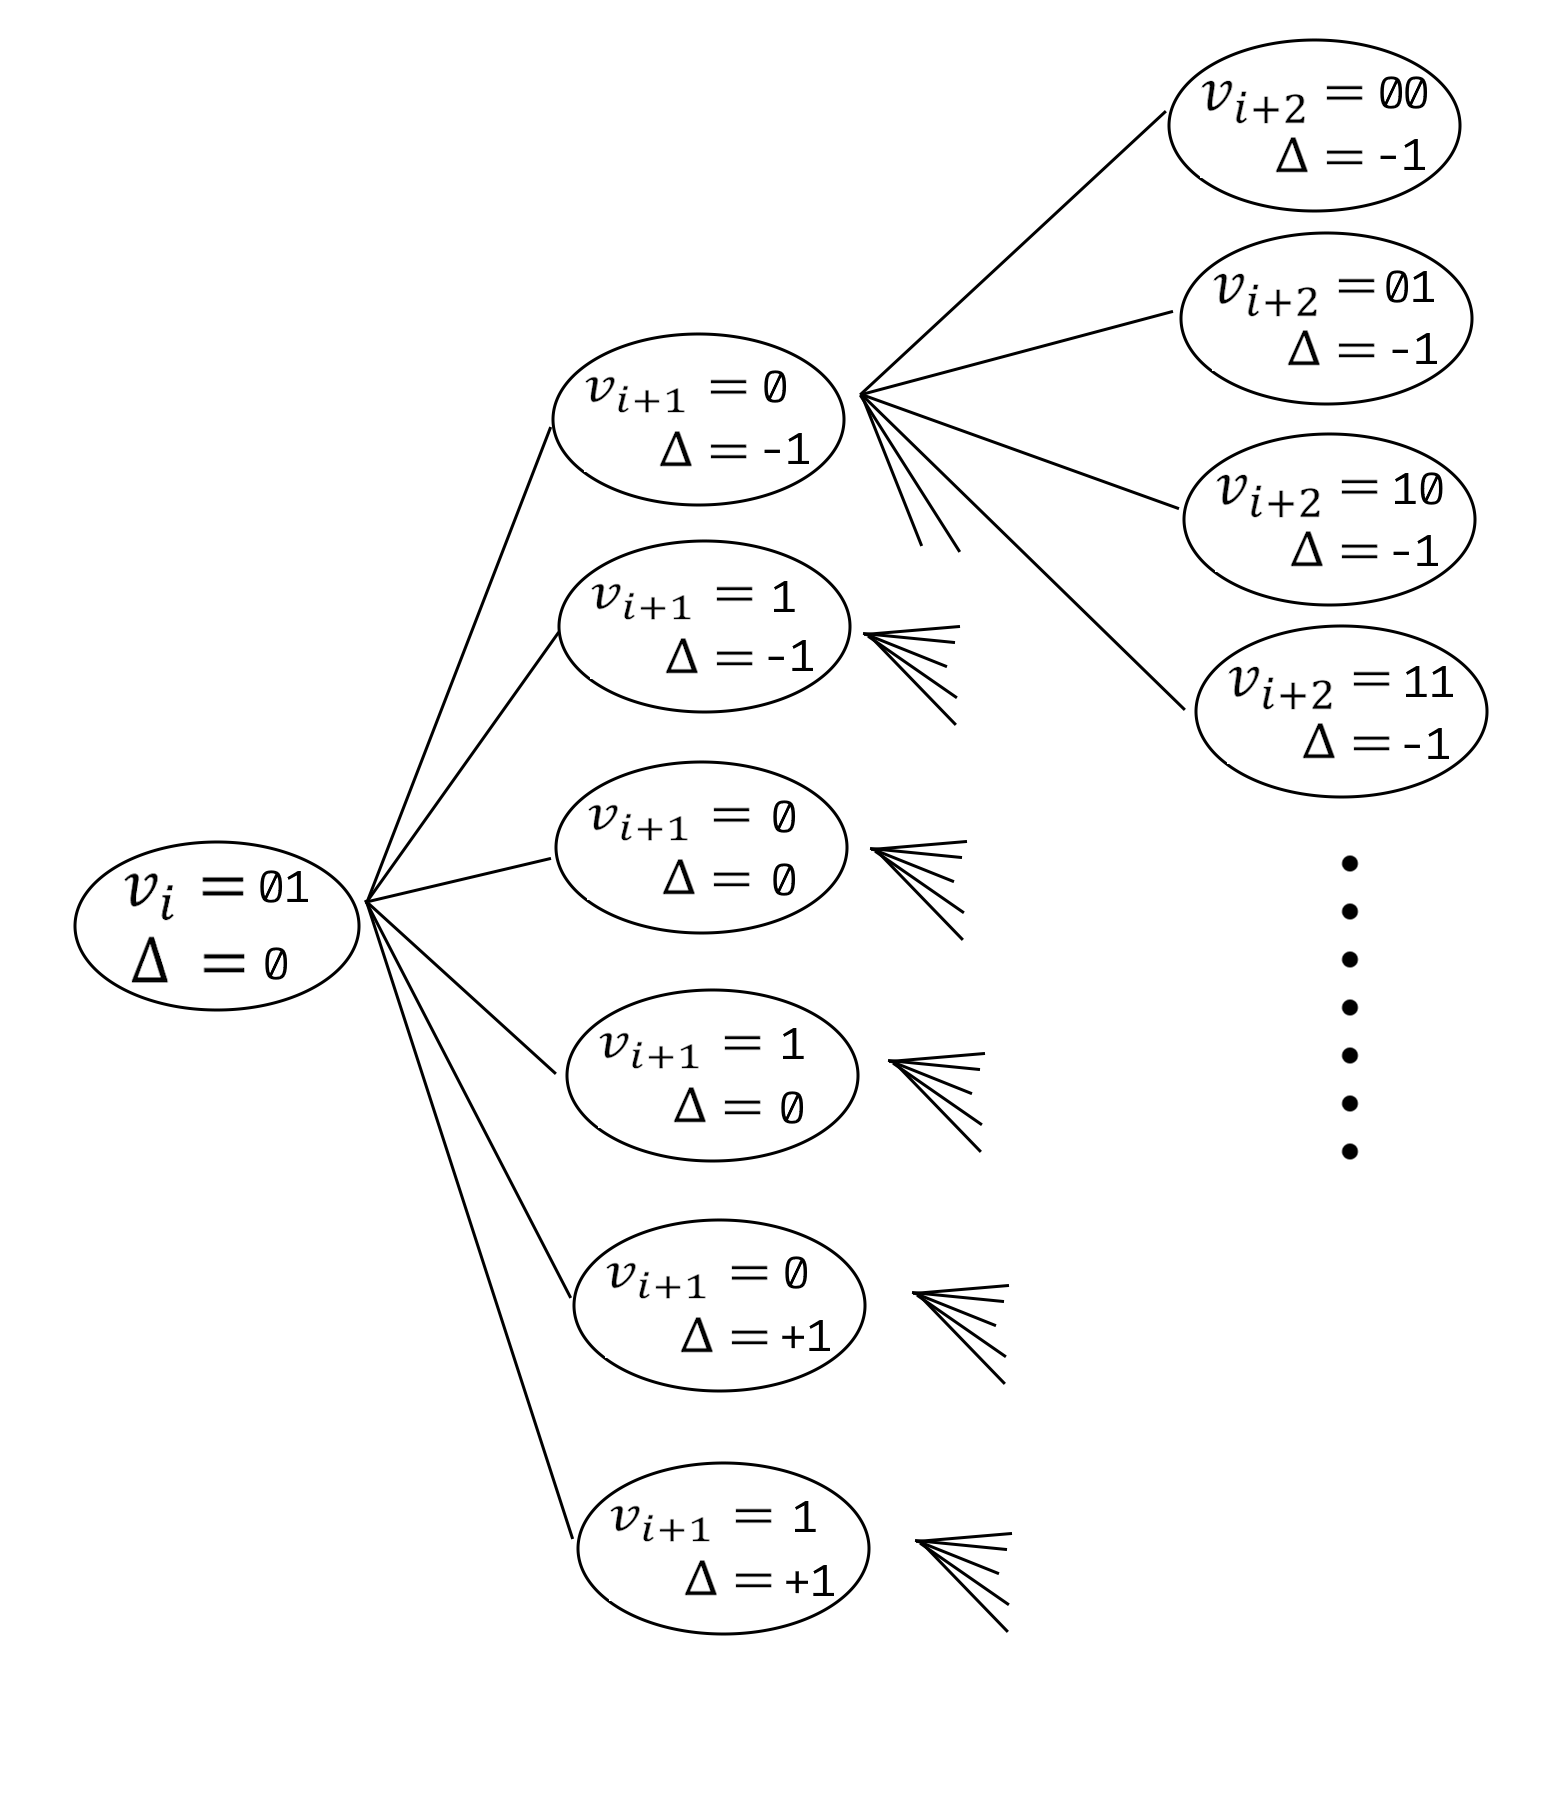
\includegraphics[width=100mm]{heap.png}
        \caption{Heap structure in HEDGES decoding}\label{fig:heap}
    \end{center}
\end{figure}
In the decoding process, candidates are first generated for all combinations of
bit group $v_i$ and skew $\Delta$, and added to the heap.
For each candidate, the predicted base $C_i$ obtained from $v_i$ via
Eq.~\eqref{encode} is compared with the actually observed base $C'_i$ for that
candidate.
If they match, a reward is added to the score; otherwise, a penalty is added.
At each step, the candidate with the minimum score is selected and expanded as
the parent for the next candidates, thereby constructing the heap.
Depending on skew, the step penalty $\Delta P$ is computed as follows using
reward $P_{\mathrm{ok}}$, substitution penalty $P_{\mathrm{sub}}$, insertion
penalty $P_{\mathrm{ins}}$, and deletion penalty $P_{\mathrm{del}}$:
\begin{itemize}
  \item Case $\Delta = 0$: \\ no positional shift, representing either a match
  or substitution.
  \begin{align}
    \Delta P = \begin{cases}
      P_{\mathrm{ok}} & (\text{if matched}) \\
      P_{\mathrm{sub}} & (\text{if mismatched})
    \end{cases}
  \end{align}
  \item Case $\Delta = -1$:\\ a deletion is hypothesized, so the input-base
  reference position is shifted one step backward.
  In this case, no base comparison is performed.
  \begin{align}
    \Delta P = P_{\mathrm{del}}
  \end{align}
  \item Case $\Delta = 1$: \\ a one-base insertion is hypothesized, so the
  input-base reference position is shifted one step forward.
  \begin{align}
    \Delta P = \begin{cases}
      P_{\mathrm{ins}} + P_{\mathrm{ok}} & (\text{if matched}) \\
      P_{\mathrm{ins}} + P_{\mathrm{sub}} & (\text{if mismatched})
    \end{cases}
  \end{align}
\end{itemize}
The score of each hypothesis is accumulated by adding $\Delta P$ to the parent
hypothesis score.
As a result, the correct decoding path tends to have a distinctly lower score
than incorrect paths, enabling efficient identification of the correct path.
However, for the last few bytes of a message, there are not enough subsequent
bases for penalties on wrong hypotheses to accumulate sufficiently, which
degrades decoding accuracy.
To address this issue, two bytes of zero padding called runout are appended to
the end of the message during encoding and removed during decoding.

In heap search during decoding, to prevent explosive growth in computational
complexity, a maximum heap size is imposed.
When this limit is reached, decoding failure is declared, the search is
terminated, and the remaining part of the DNA strand is marked as bit erasures.
These bit erasures are finally corrected by the RS outer code.

\section{Nanopore Sequencers and Basecallers} \label{nanopore}
A nanopore sequencer analyzes DNA base sequences by exploiting the fact that DNA
is charged in solution and driving DNA through a protein pore called a nanopore
via electrophoresis \cite{Amarasinghe2020,Dorey2024}.
Figure~\ref{fig:nanopore} illustrates the process of DNA analysis by a
nanopore sequencer.
Multiple nanopore proteins are arranged on the sensor substrate called a flow
cell.
Each pore has a diameter of about 1 nm, allowing only a single DNA strand to
pass through.
The flow cell is filled with an electrolyte containing potassium chloride.
Because DNA is negatively charged in solution, applying voltage causes
electrophoretic motion in the direction of the electric field.
This controls DNA movement and guides molecules into nanopores.
The guided DNA is unwound from double-stranded to single-stranded DNA by an
enzyme called helicase while being regulated to pass through the nanopore at a
controlled speed.
As DNA passes through the pore, it interferes with ionic flow inside the pore,
causing changes in ionic current.
Because current changes depend on the sequence of bases currently passing
through the nanopore, DNA base sequences can be determined by analyzing current
signals.
\begin{figure}
    \begin{center}
        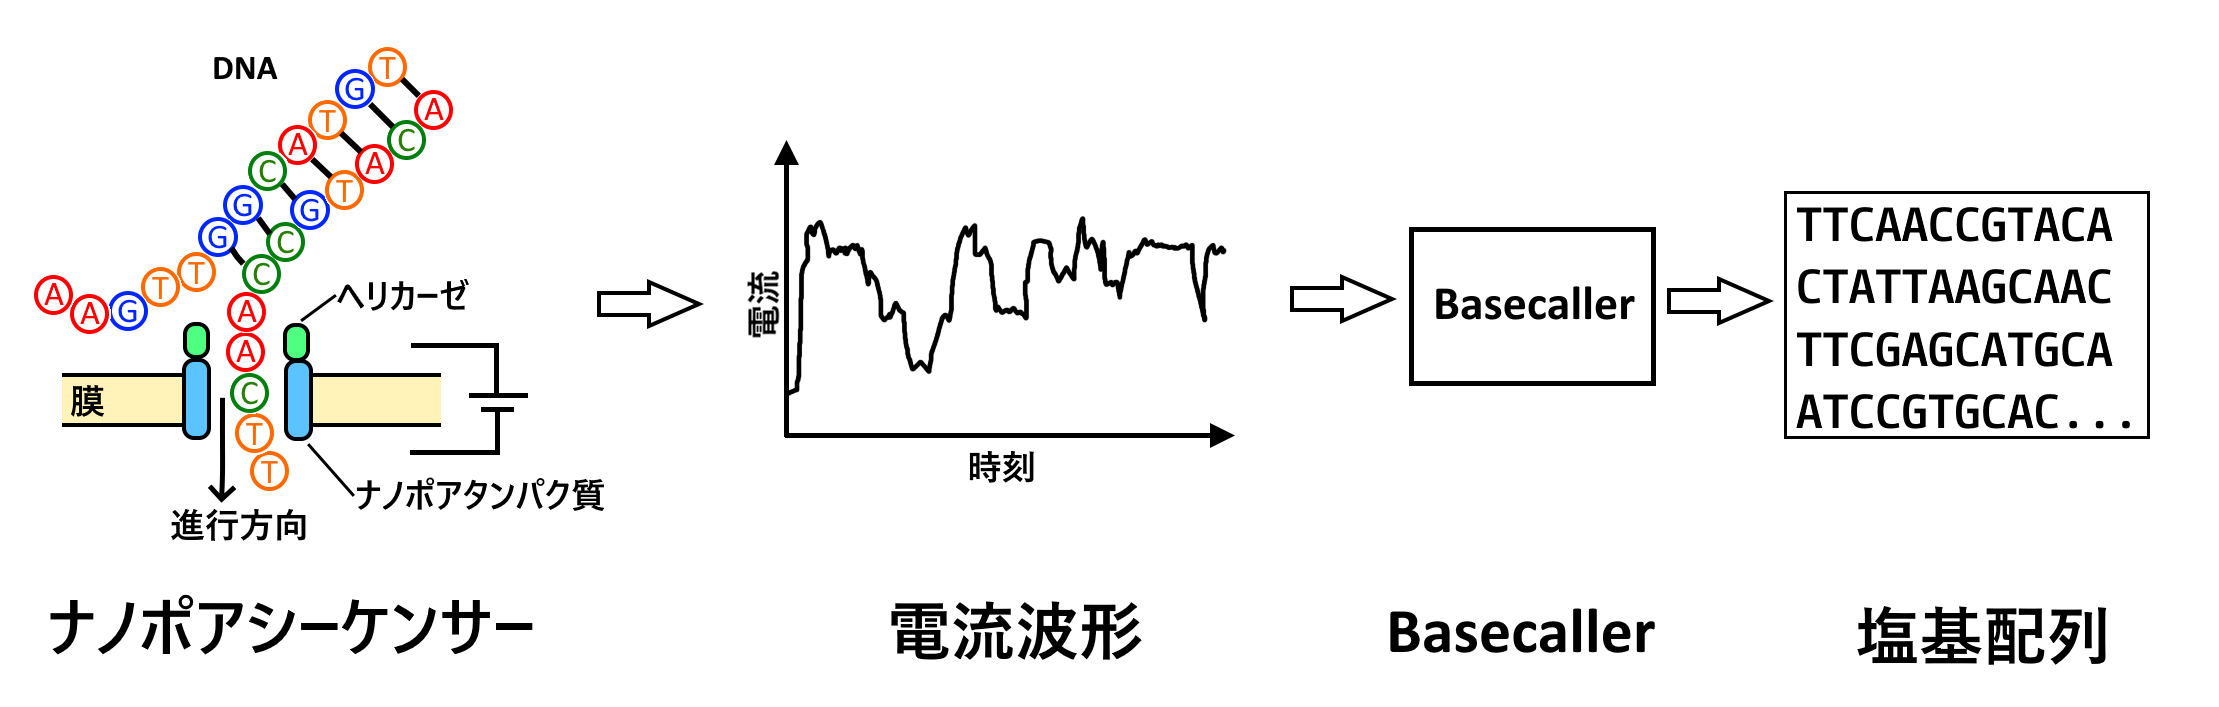
\includegraphics[width=150mm]{nanopore.png}
        \caption{Principle and procedure of nanopore sequencing}\label{fig:nanopore}
    \end{center}
\end{figure}

The process of determining base sequences from electrical signals is called
basecalling, and is performed by machine-learning models called basecallers.
Figure~\ref{fig:bonito} shows an overview of the Bonito basecaller architecture
used in this study \cite{bonito}.
In Bonito, a CNN is first applied to input current signals to extract features.
Next, an LSTM captures long-range dependencies in the current signals and
extracts temporal features.
Then, in the CTC output layer, a linear layer is applied to the LSTM output to
produce score sequences over the label set (N, A, C, G, T), where N denotes
blank.
Beam search is applied to this score sequence to determine the final base
sequence.
At this stage, the following process, called collapse, is applied to the label
sequence:
\begin{enumerate}
  \item Merge consecutive identical labels into one.
  \item Remove blank labels (N).
\end{enumerate}
For example, the label sequence ``AANNCCGNGGGTT'' is converted to ``ACGGT''.
\begin{figure}
    \begin{center}
        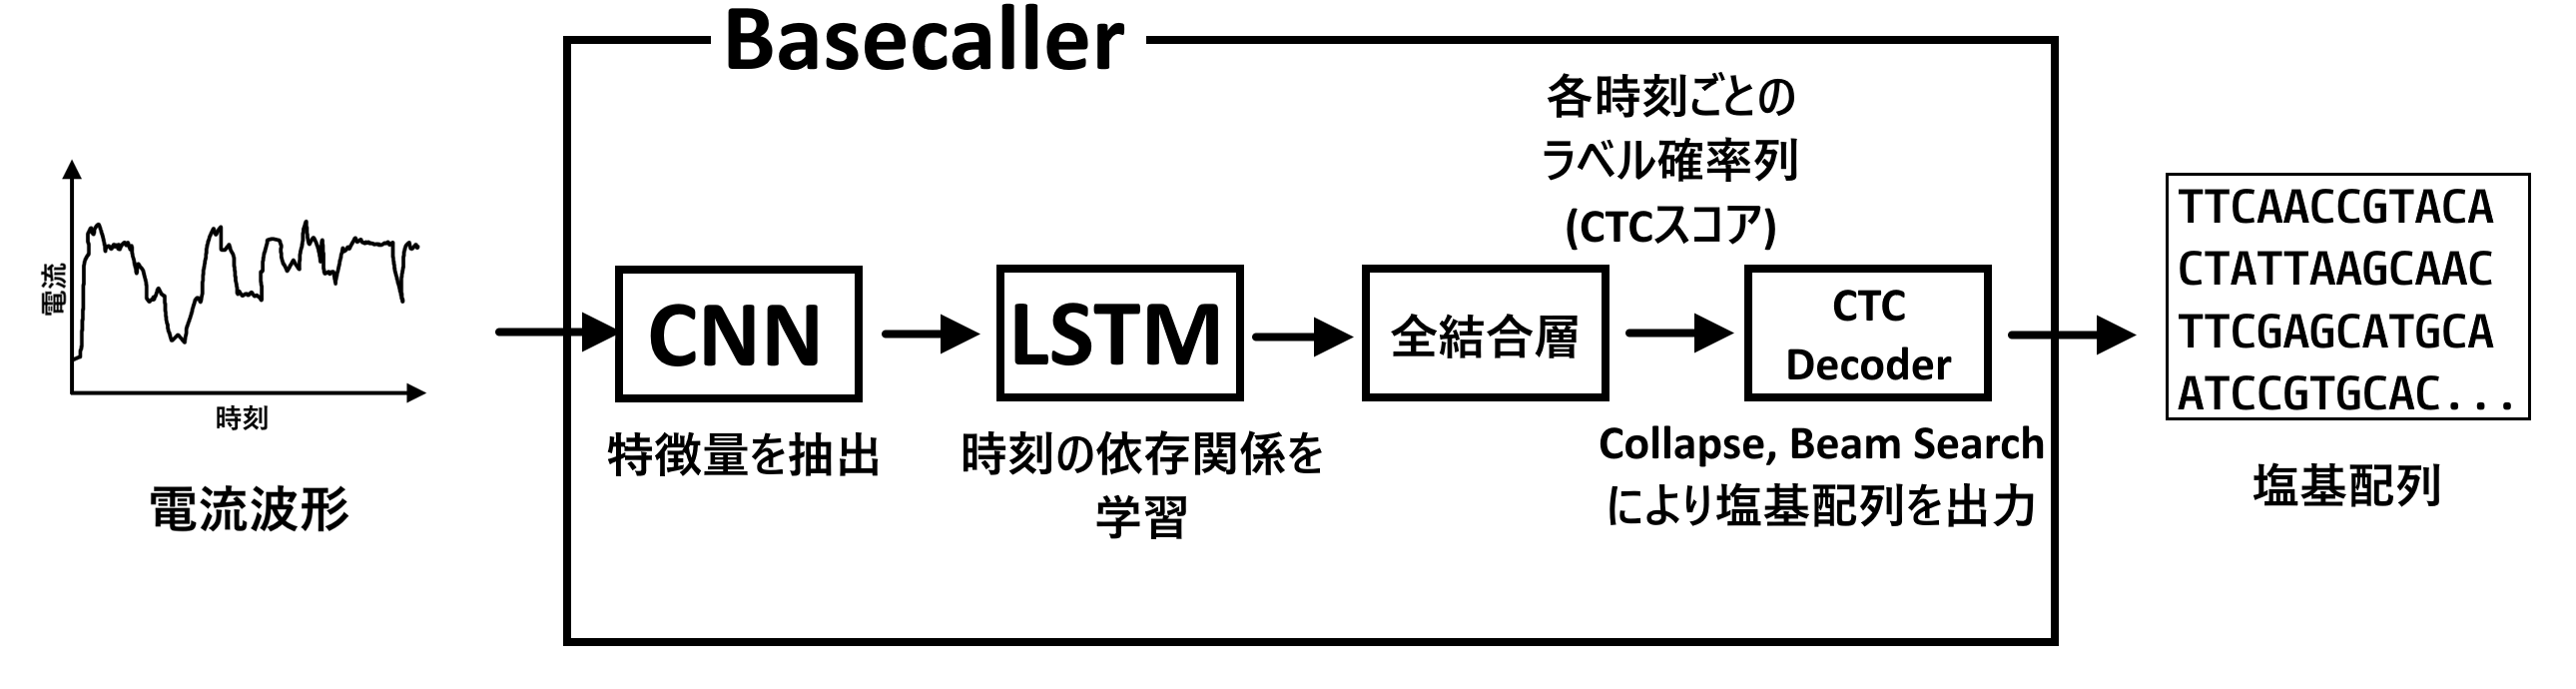
\includegraphics[width=150mm]{architecture.png}
        \caption{Overview of the Bonito architecture}\label{fig:bonito}
    \end{center}
\end{figure}

Advantages of nanopore sequencers for DNA storage readout include direct
analysis of long DNA sequences, ranging from several hundred bp to several
million bp, and high-speed sequencing.
On the other hand, controlling DNA translocation speed with helicase is
difficult, and basecallers may fail to infer base sequences accurately.
Therefore, nanopore sequencers are known to have lower read accuracy than SBS,
and error-correcting code design is especially important for DNA storage systems
using nanopore sequencers \cite{Amarasinghe2020,Dorey2024}.

\section{Limitations of Existing Methods and Research Objective} \label{sec:problem}
The main limitations of the method reported in \cite{HEDGES} are as follows:
\begin{itemize}
  \item Existing studies do not optimize rewards and penalties based on
  statistical output characteristics when bases are read using nanopore
  sequencers.
  \item Because the input to the existing HEDGES decoder is a base sequence,
  decoding does not utilize the per-time-step probability distribution over
  bases output by the basecaller.
  \item In the existing HEDGES encoding/decoding method, the search complexity
  can explode for long base sequences, making it easier to hit the heap limit
  and cause decoding failure, which degrades decoding accuracy.
\end{itemize}
In this study, we propose an error-correction method for DNA storage assuming
readout with nanopore sequencers.
For rewards and penalties in HEDGES decoding, we optimize them by considering
statistical readout characteristics, such as error occurrence probabilities and
transition probabilities of each base under nanopore sequencing.
By also incorporating base probability distributions output by the basecaller
into rewards and penalties, we aim to reduce search complexity and improve
decoding accuracy.
Furthermore, we propose a method in the encoding process to suppress accuracy
degradation when handling long DNA sequences.
We evaluate the performance of these proposed methods through simulation.

\chapter{Error Correction Method Assuming Readout by Nanopore Sequencers}\label{proposed_method}
\section{Improving Search Efficiency in Decoding} \label{optimization}
This section proposes a method to optimize rewards and penalties in decoding by
considering both the statistical readout characteristics of nanopore
sequencers and the per-time-step base probability distributions in basecaller
outputs, in order to improve search efficiency during decoding.
First, we describe modeling of nanopore readout characteristics and treatment
of CTC outputs from the basecaller. Then, we explain how these are reflected in
reward and penalty calculation.

\subsection{Modeling Readout Characteristics of Nanopore Sequencers} \label{stat_model}
To model readout characteristics of nanopore sequencers, we first construct a
transition matrix representing statistical error rates.
When both the true base sequence and the post-readout base sequence are known,
the two sequences can be compared using sequence alignment to identify matched
regions and positions where various errors occur \cite{GOTOH1982705}.
In aligned sequences, matched base pairs represent correct readout, mismatched
pairs represent substitution errors, and bases aligned with gaps represent
insertion/deletion errors.
From such alignment information, each event in DNA readout, namely correct
readout and occurrences of substitution, insertion, and deletion errors, can be
represented as transitions among five labels $\{N,A,C,G,T\}$ consisting of
four bases plus blank (N).

Using this representation, the statistical readout characteristics of nanopore
sequencers are described by the following matrix $\bm{T}$:
\begin{align}
  \bm{T} = \begin{bmatrix}
    0 & p_{AN} & p_{CN} & p_{GN} & p_{TN} \\
    p_{NA} & p_{AA} & p_{CA} & p_{GA} & p_{TA} \\
    p_{NC} & p_{AC} & p_{CC} & p_{GC} & p_{TC} \\
    p_{NG} & p_{AG} & p_{CG} & p_{GG} & p_{TG} \\
    p_{NT} & p_{AT} & p_{CT} & p_{GT} & p_{TT} \\
  \end{bmatrix}
\end{align}
Each element in this matrix represents the probability of correct readout or
occurrence of substitution/insertion/deletion errors when a sufficiently long
DNA sequence containing A, C, G, and T in equal proportions is read by a
nanopore sequencer.
For $X,Y \in \{A,C,G,T\}$:
\begin{itemize}
  \item $p_{XX}$: probability that base X is correctly read.
  \item $p_{XY}$: probability that base X is substituted by base Y.
  \item $p_{XN}$: probability that base X is deleted.
  \item $p_{NY}$: probability that base Y is inserted.
\end{itemize}
The sum of all elements of $\bm{T}$ is 1.
We define $\bm{P}_{\mathrm{STATS}}$ as the matrix obtained by taking the
natural logarithm of each element of $\bm{T}$ except the first-row/first-column
element and multiplying by $-1$. This matrix is used later to compute rewards
and penalties.

\subsection{Treatment of CTC Output} \label{ctc_output}
As described in Section~\ref{nanopore}, a basecaller usually outputs final base
sequences by applying beam search to CTC outputs. In the proposed method,
however, the basecaller does not finalize base sequences and instead outputs the
CTC score sequence directly.
Also, as described in Section~\ref{hedges_decoding}, while the existing HEDGES
decoder uses base sequences as input, the proposed method uses CTC score
sequences as input (Fig.~\ref{fig:optim}). This enables incorporation of
per-time-step base probability distributions into decoding.
\begin{figure}
    \begin{center}
        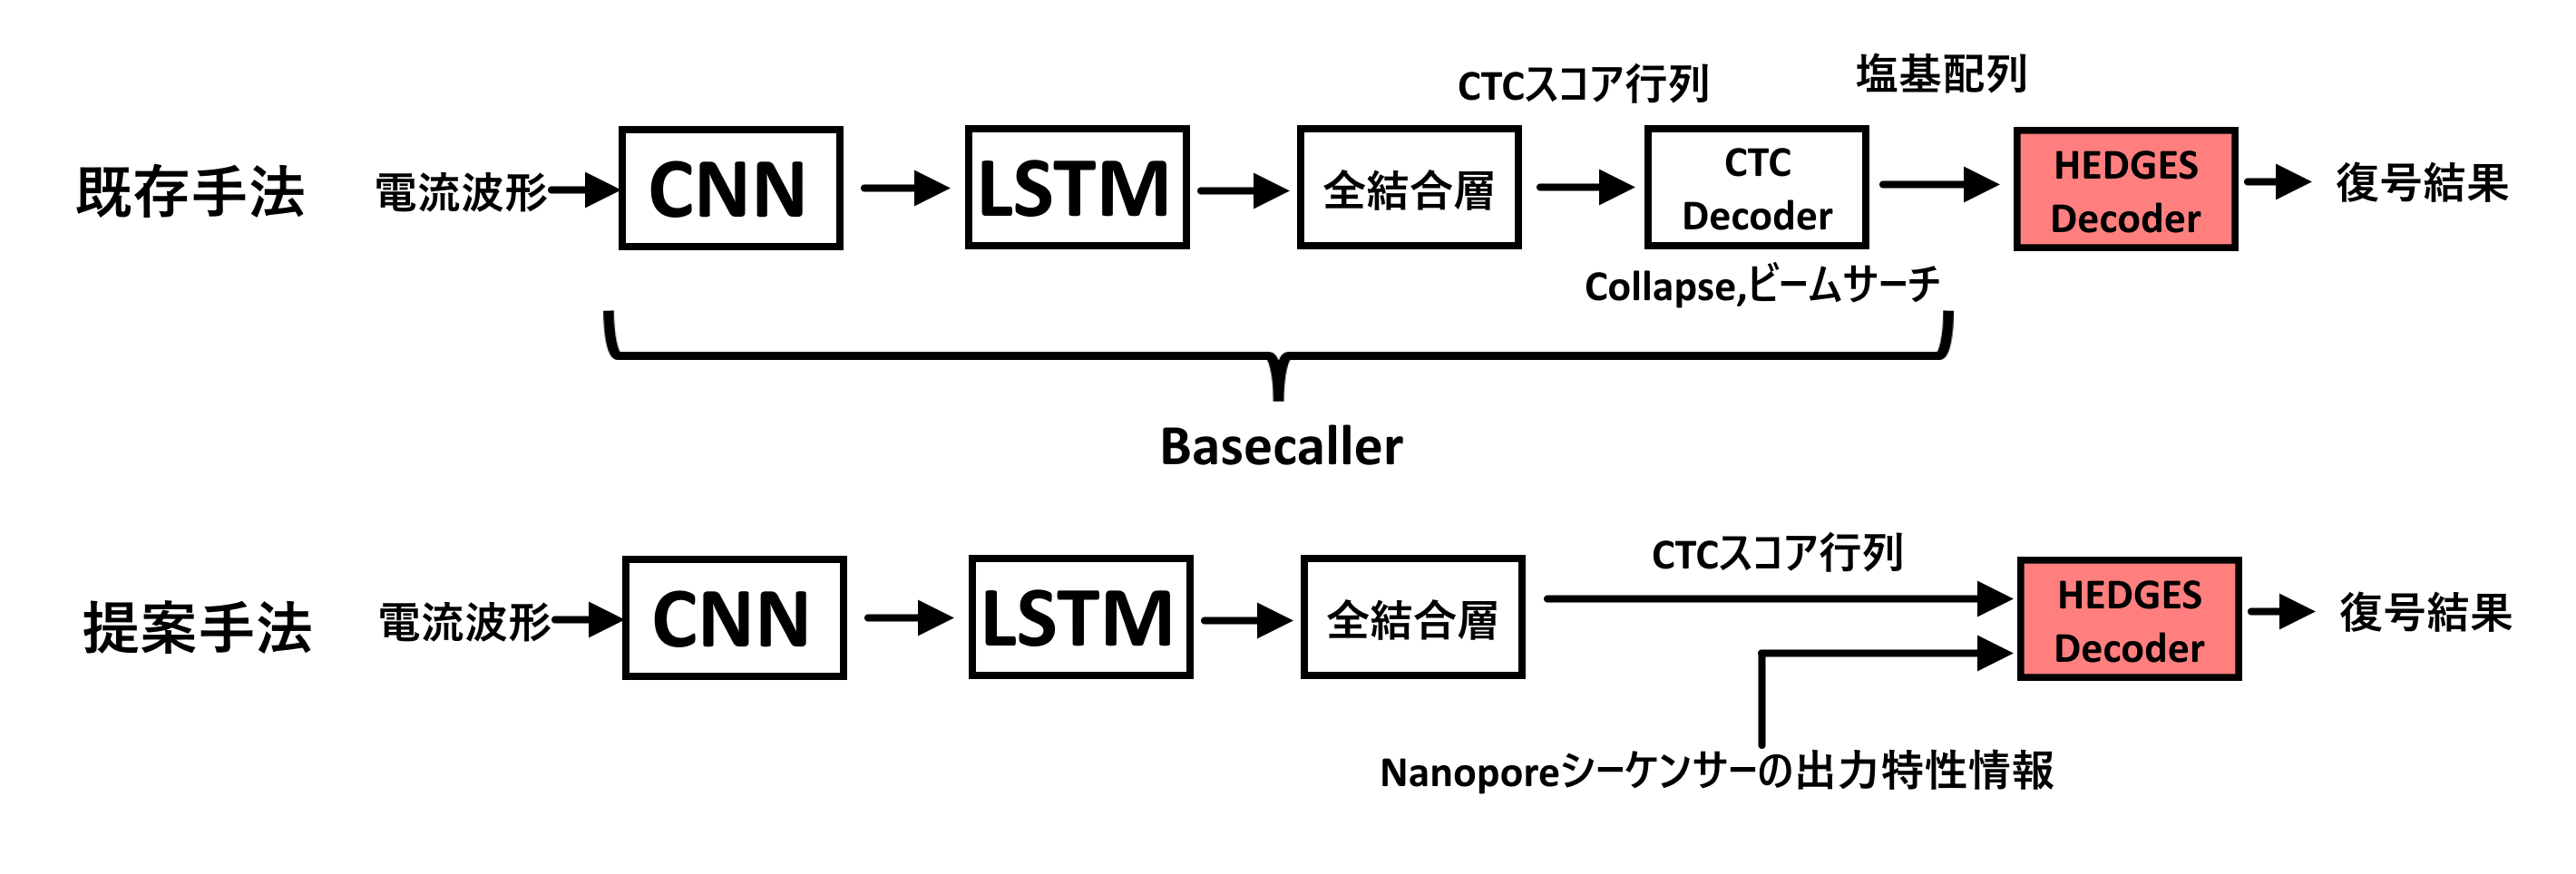
\includegraphics[width=150mm]{optim.png}
        \caption{Overview of the proposed method}\label{fig:optim}
    \end{center}
\end{figure}

Assume the CTC output is given as an $L\times 5$ matrix $\bm{S}$, where $L$ is
the time-series length dependent on the input current-signal length, and each
row represents output probabilities over the five labels $\{N,A,C,G,T\}$ at
each time step.
Applying the following operations, corresponding to collapse in
Section~\ref{nanopore}, yields $\bm{S}'$:
\begin{enumerate}
  \item For consecutive rows in $\bm{S}$ whose maximum-probability label is the
  same, average the probabilities for each label and merge them into one row.
  \item Remove rows in $\bm{S}'$ whose maximum-probability label is blank (N).
\end{enumerate}
% なお，これにより得られた行列$\bm{S}'$の各行で確率が最大となる塩基を選択することで
% 得られる塩基配列は，通常のベースコーラーの最終層でのビームサーチにおいてビーム幅を1と
% した場合のベースコール結果に相当する．
Let $\bm{P}_{\mathrm{CTC}}$ be the matrix obtained by taking the natural
logarithm of each element in $\bm{S}'$ and multiplying by $-1$.
Elements of $\bm{P}_{\mathrm{CTC}}$ represent score values based on
probabilities that each base or blank is output at each time step.
As described in Section~\ref{hedges_decoding}, the existing HEDGES decoding
algorithm determines rewards and penalties by comparing the base predicted from
Eq.~\eqref{encode} with the corresponding input base.
In the proposed method, rewards and penalties are determined using scores
retrieved from $\bm{P}_{\mathrm{CTC}}$ based on the output probability of the
predicted base for each hypothesis.

\subsection{Optimization of Rewards and Penalties} \label{reward_penalty_optimization}
In the existing method, reward $P_{\mathrm{ok}}$ and penalties
$P_{\mathrm{sub}}$, $P_{\mathrm{ins}}$, and $P_{\mathrm{del}}$ for
substitution, insertion, and deletion errors are fixed values.
In this study, we propose new reward/penalty terms
$P'_{\mathrm{ok}}$, $P'_{\mathrm{sub}}$, $P'_{\mathrm{ins}}$, and
$P'_{\mathrm{del}}$ that incorporate nanopore readout characteristics and
basecaller CTC outputs described in Sections~\ref{stat_model} and
\ref{ctc_output}, and define them as follows:
\begin{equation}
  \begin{split}
    P'_{\mathrm{ok}} = P_{\mathrm{ok}} &+ \alpha_{\mathrm{ok}}(\bm{P}_{\mathrm{STATS}}(x_{\mathrm{hypo}}, x_{\mathrm{max}}(i))-\mu_{\mathrm{STATS}\_\mathrm{ok}}) \label{opt1} \\ 
     &+ \beta_{\mathrm{ok}}(\bm{P}_{\mathrm{CTC}}(i, x_{\mathrm{hypo}})-\mu_{\mathrm{CTC}\_\mathrm{ok}}) 
  \end{split}
\end{equation}
\begin{equation}
  \begin{split}
    P'_{\mathrm{sub}} = P_{\mathrm{sub}} &+ \alpha_{\mathrm{sub}}(\bm{P}_{\mathrm{STATS}}(x_{\mathrm{hypo}}, x_{\mathrm{max}}(i))-\mu_{\mathrm{STATS}\_\mathrm{sub}}) \label{opt2} \\
    &+ \beta_{\mathrm{sub}}(\bm{P}_{\mathrm{CTC}}(i, x_{\mathrm{hypo}})-\mu_{\mathrm{CTC}\_\mathrm{sub}})
  \end{split}
\end{equation}
\begin{equation}
  \begin{split}
    P'_{\mathrm{ins}} = P_{\mathrm{ins}} &+ \alpha_{\mathrm{ins}}(\bm{P}_{\mathrm{STATS}}(N, x_{\mathrm{max}}(i-1))-\mu_{\mathrm{STATS}\_\mathrm{ins}}) \label{opt3}\\
    &+ \beta_{\mathrm{ins}}(\bm{P}_{\mathrm{CTC}}(i-1, x_{\mathrm{hypo}})-\mu_{\mathrm{CTC}\_\mathrm{ins}})
  \end{split}
\end{equation}
\begin{equation}
  \begin{split}
    P'_{\mathrm{del}} = P_{\mathrm{del}} &+ \alpha_{\mathrm{del}}(\bm{P}_{\mathrm{STATS}}(x_{\mathrm{hypo}}, N)-\mu_{\mathrm{STATS}\_\mathrm{del}}) \label{opt4}
  \end{split}
\end{equation}
Here, $x_{\mathrm{hypo}}$ denotes the base output from a hypothesis bit
sequence, and $i$ denotes the row index of $\bm{P}_{\mathrm{CTC}}$ referenced
by that hypothesis.
$x_{\mathrm{max}}(i)$ denotes the base with maximum output probability in the
$i$-th row of $\bm{P}_{\mathrm{CTC}}$.
$\bm{P}_{\mathrm{STATS}}(X,Y)\quad(X,Y\in \{N,A,C,G,T\})$ denotes the score
corresponding to transition from label $X$ to label $Y$ in
$\bm{P}_{\mathrm{STATS}}$.
$\bm{P}_{\mathrm{CTC}}(i,X)$ denotes the score of label $X$ in row $i$ of
$\bm{P}_{\mathrm{CTC}}$.
$\mu_{\mathrm{STATS}\_\mathrm{ok}}$,
$\mu_{\mathrm{STATS}\_\mathrm{sub}}$,
$\mu_{\mathrm{STATS}\_\mathrm{ins}}$,
and $\mu_{\mathrm{STATS}\_\mathrm{del}}$ denote the expected values of
$\bm{P}_{\mathrm{STATS}}$ scores when correct readout, substitution,
insertion, and deletion errors occur, respectively.
% すなわち
% \begin{align}
%   \mu_{\mathrm{STATS}\_\mathrm{ok}} &= \dfrac{\displaystyle \sum_{X \in \{A,C,G,T\}} p_{XX} \bm{P}_{\mathrm{STATS}}(X,X)}{\displaystyle \sum_{X \in \{A,C,G,T\}} p_{XX}} \\
%   \mu_{\mathrm{STATS}\_\mathrm{sub}} &= \dfrac{\displaystyle \sum_{X,Y \in \{A,C,G,T\}, X \neq Y} p_{XY} \bm{P}_{\mathrm{STATS}}(X,Y)}{\displaystyle \sum_{X,Y \in \{A,C,G,T\}, X \neq Y} p_{XY}} \\
%   \mu_{\mathrm{STATS}\_\mathrm{ins}} &= \dfrac{\displaystyle \sum_{Y \in \{A,C,G,T\}} p_{NY} \bm{P}_{\mathrm{STATS}}(N,Y)}{\displaystyle \sum_{Y \in \{A,C,G,T\}} p_{NY}} \\
%   \mu_{\mathrm{STATS}\_\mathrm{del}} &= \dfrac{\displaystyle \sum_{X \in \{A,C,G,T\}} p_{XN} \bm{P}_{\mathrm{STATS}}(X,N)}{\displaystyle \sum_{X \in \{A,C,G,T\}} p_{XN}}
% \end{align}
% である．
$\mu_{\mathrm{CTC}\_\mathrm{ok}}$,
$\mu_{\mathrm{CTC}\_\mathrm{sub}}$,
and $\mu_{\mathrm{CTC}\_\mathrm{ins}}$ denote the statistical expected values
of scores in $\bm{P}_{\mathrm{CTC}}$ corresponding to correct readout,
substitution error, and insertion error, respectively.
Reward and penalties are calculated by adding normalized correction terms,
whose expectations are zero, to the fixed values
$P_{\mathrm{ok}}$, $P_{\mathrm{sub}}$, $P_{\mathrm{ins}}$, and
$P_{\mathrm{del}}$.
Each correction term is multiplied by adjustment parameters
$\alpha_{\mathrm{ok}}$, $\alpha_{\mathrm{sub}}$, $\alpha_{\mathrm{ins}}$,
$\alpha_{\mathrm{del}}$, $\beta_{\mathrm{ok}}$, $\beta_{\mathrm{sub}}$, and
$\beta_{\mathrm{ins}}$.
The fixed penalties and the weights of correction terms are optimized by
simulation. Details of constant settings and parameter optimization are
described in the appendix.
% まず，仮説のビット列から出力される塩基を$x_{\mathrm{hypo}}$とする．
% また，仮説が参照する$\bm{P}_{\mathrm{CTC}}$の行番号を$i$とする．
% このとき，$\bm{P}_{\mathrm{CTC}}$の$i$行目において出力確率が最大となる塩基を
% $x_{\mathrm{max}}(i)$とする．

\section{Improved Encoding Algorithm for Long Reads} \label{long_read_encoding}
As described in Section~\ref{sec:problem}, in the existing HEDGES
encoding/decoding method, decoding accuracy decreases as DNA sequence length
increases.
This is because when the number of hypotheses reaches the heap-size limit in
the decoding algorithm, decoding failure is declared and all subsequent bits are
treated as erasures. Therefore, the failure rate increases with sequence
length.
This section proposes an improved encoding/decoding method that suppresses
accuracy degradation when handling long DNA sequences.

In the HEDGES encoder, each output base $C_i$ corresponding to bit group $v_i$
is determined recursively by Eq.~\eqref{encode} using a hash function based on
DNA strand ID, bit position, and recent bit history.
Therefore, for example, if a burst error occurs at some position of a DNA
strand, the impact propagates to decoding of subsequent bases, making correct
path search difficult.
To address this, the proposed method divides long base sequences into
400\,nt segments as shown in Fig.~\ref{fig:segment}, and initializes the bit
position $I_i$ and recent-bit information $B_i$ to zero at the beginning of
each segment during encoding.
To identify boundaries between adjacent segments, a known separator sequence of
about 10 bases with a specific pattern is inserted between segments.
A separator pattern is selected to avoid homopolymers and maintain GC content
around 50\%. In this study, "GTACTGCATG" is used as the separator.

During decoding, separator positions are first detected by the following
procedure:
\begin{enumerate}
  \item Set $n=l_{\mathrm{p}} + l_{\mathrm{seg}}$, where $l_{\mathrm{p}}$
  denotes primer length and $l_{\mathrm{seg}}$ denotes segment length.
  \item For each integer $k$ satisfying $n-30<k<n+30$, compute
  $S_{\mathrm{match}}(k)$ by the following equation, and select the $k$ that
  minimizes $S_{\mathrm{match}}(k)$ as the separator position, denoted $k'$.
  \begin{align}
    S_{\mathrm{match}}(k) = \sum_{j=0}^{l_{\mathrm{sep}}-1} \bm{P}_{\mathrm{CTC}}(k+j, S_j) \label{eq:separator_detection}
  \end{align}
  Here, $S_j$ denotes the $j$-th base of the separator sequence, and
  $l_{\mathrm{sep}}$ denotes separator length.
  \item Set $n=k' + l_{\mathrm{sep}}+l_{\mathrm{seg}}$.
  \item Repeat steps 2 and 3 to detect separator positions for all segments.
\end{enumerate}
After separator positions are identified, the decoding algorithm described in
Section~\ref{hedges_decoding} is applied to each segment.
At the beginning of each segment, $I_i$ and $B_i$ are reset to zero and the
heap is reinitialized before decoding.
This suppresses decoding failure caused by exceeding heap-size limits, and even
if a decoding failure occurs, its impact is confined within a segment so that
decoding can resume from the next segment.
\begin{figure}
    \begin{center}
        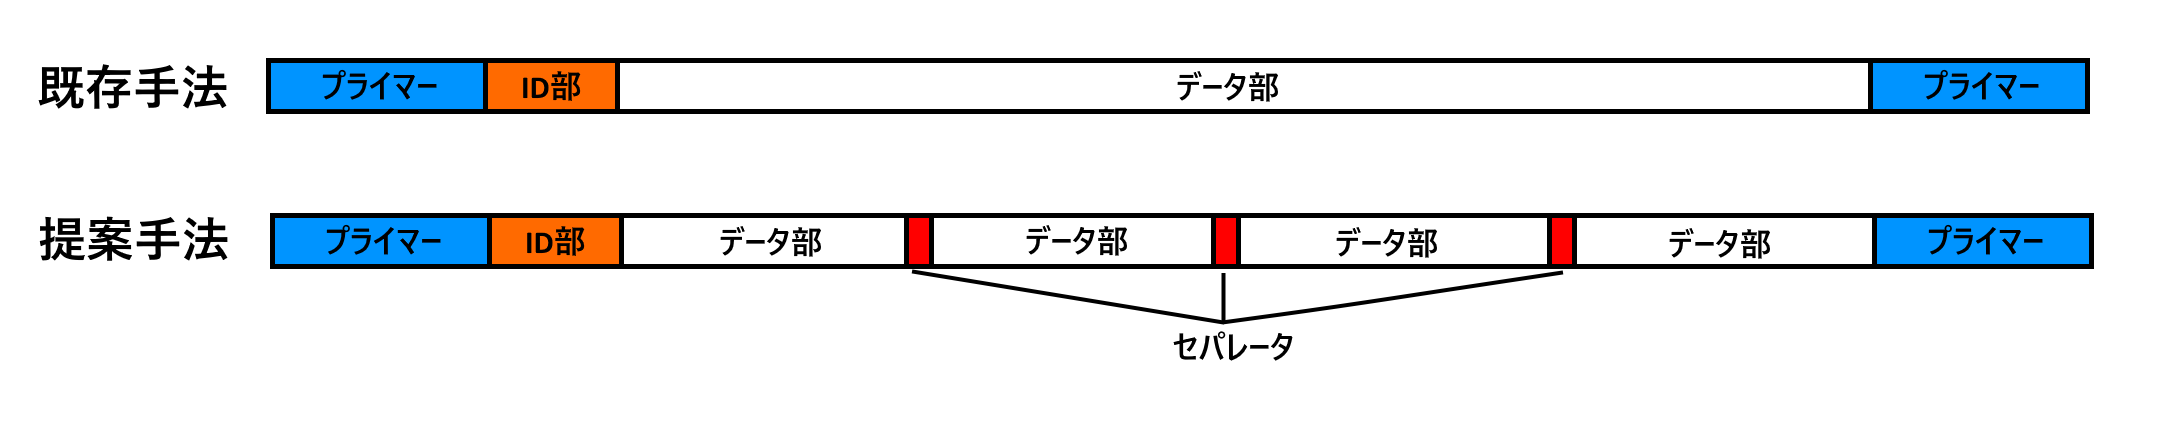
\includegraphics[width=150mm]{segment.png}
        \caption{Encoding scheme of the proposed method}\label{fig:segment}
    \end{center}
\end{figure}

\chapter{Simulation Evaluation} \label{simulation}
In this chapter, we evaluate the performance of the proposed methods through
simulation.
In Section~\ref{sim1}, we measure the number of search operations and decoding
accuracy when using the reward/penalty optimization proposed in
Section~\ref{optimization}, and evaluate its effectiveness by comparison with
the existing method.
In Section~\ref{sim2}, we measure decoding accuracy when using the improved
encoding/decoding algorithm for long reads proposed in
Section~\ref{long_read_encoding}, and evaluate its effectiveness by comparison
with the existing method.

\section{Decoding Search Efficiency Improvement} \label{sim1}
\subsection{Experimental Method}
Figure~\ref{fig:sim1} shows an overview of the experimental procedure used to
evaluate, through simulation, the performance of the reward/penalty
optimization method proposed in Section~\ref{optimization}.
\begin{figure}
    \begin{center}
        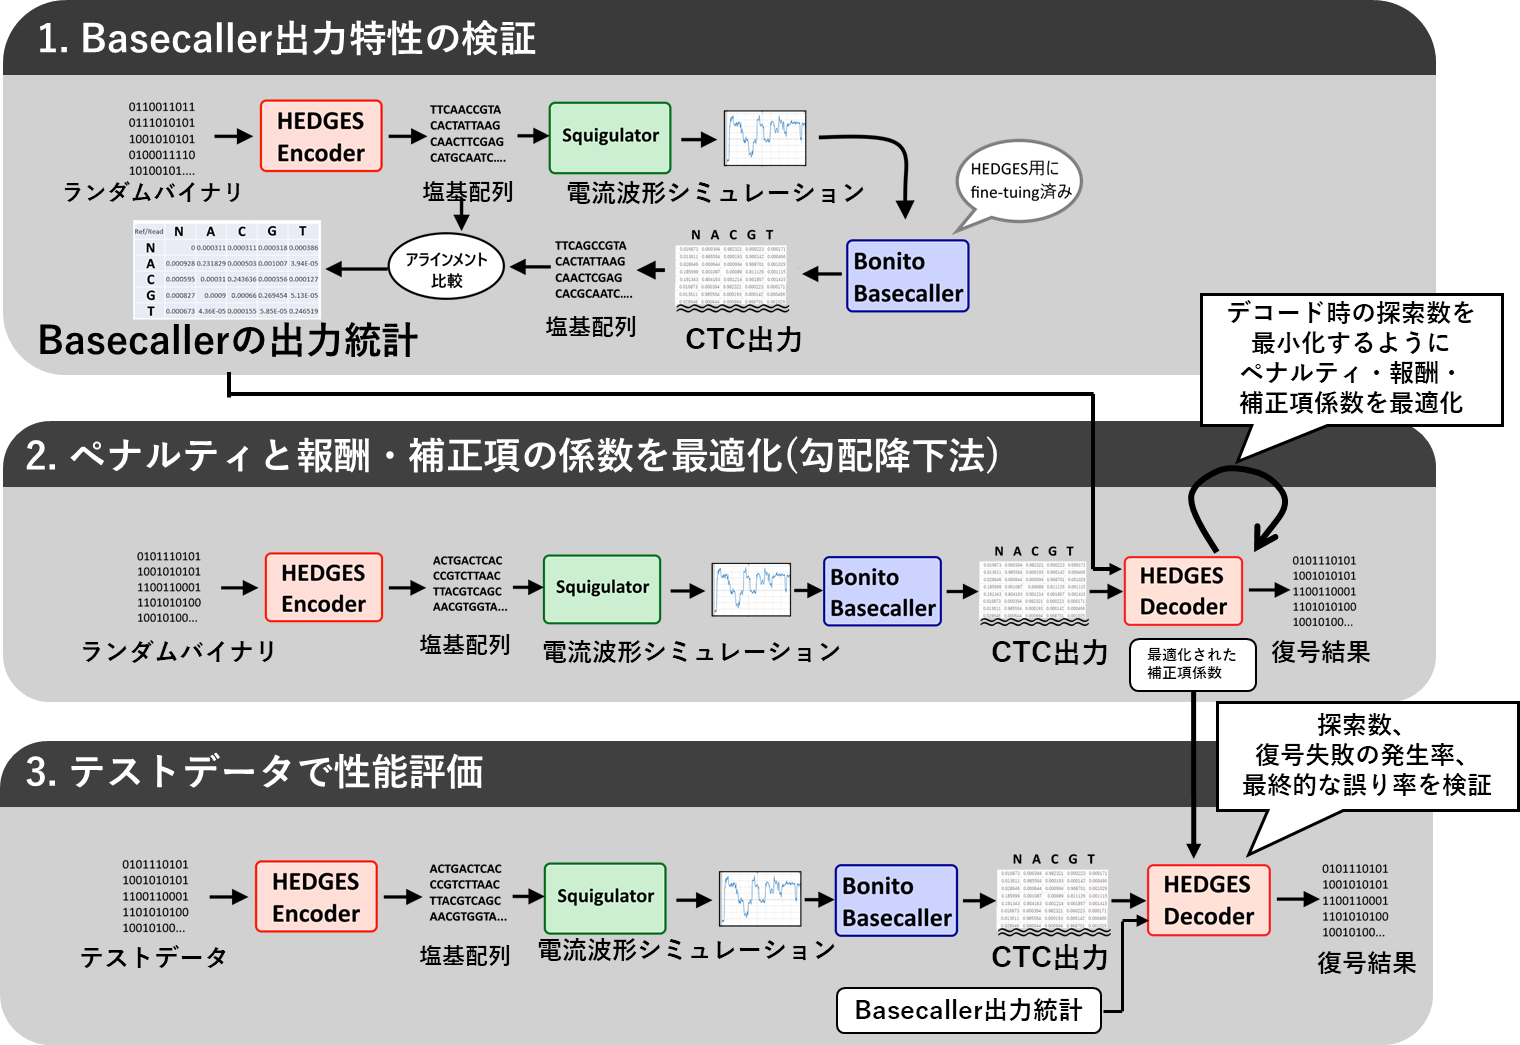
\includegraphics[width=150mm]{simu1.png}
        \caption{Overview of the simulation procedure}\label{fig:sim1}
    \end{center}
\end{figure}
As a preliminary experiment, we evaluated nanopore readout characteristics by
simulation and obtained the matrix $\bm{P}_{\mathrm{STATS}}$.
Next, in encoding/decoding simulations using random binary data, we optimized
the parameters of the correction terms in Eqs.~\eqref{opt1}--\eqref{opt4}
using gradient descent, with the number of heap search operations during
decoding as the objective function.
Parameter optimization was performed independently for multiple coding rates,
under three settings: using only correction terms based on nanopore output
characteristics, using only correction terms based on CTC output, and using
both correction terms.
Detailed procedures and conditions of these preliminary experiments are
described in the appendix.

Using the optimal parameters obtained in the preliminary experiments, we
evaluated decoding performance of the proposed methods.
First, binary test data were encoded by HEDGES, and current waveforms for the
resulting DNA strands were generated using a simulator called
Squigulator\cite{squigulator} for nanopore sequencing.
Next, basecalling was performed on the simulated current waveforms using
Bonito.
At this stage, we output not only the final base sequence but also the CTC
score matrix before CTC decoding.
Using these basecalling results, we performed decoding with the existing and
proposed methods, and measured the number of heap searches, the number of bit
erasures due to decoding failure, and the final bit error rate after RS
decoding.
In decoding with the existing method, the input is the base sequence output by
the basecaller.
In decoding with the proposed method, the input is the CTC score matrix, and
three cases were evaluated: using only correction terms based on nanopore
readout characteristics, using only correction terms based on CTC output, and
using both correction terms.
This end-to-end simulation from binary-data encoding to decoding was conducted
for multiple coding rates.

\subsection{Experimental Conditions}
As test binary data, we used the full text of Kokoro by Natsume Soseki
(UTF-8), obtained from Aozora Bunko, with ruby annotations (text enclosed by
《...》) removed using regular expressions\cite{kokoro}.
The data size is 481158 bytes.
This binary data was encoded by HEDGES at coding rates
$0.75,0.60,0.50,0.33$, with a base length of 400\,nt.
For nanopore-current simulation using Squigulator, we used parameter settings
assuming a MinION R9.4.1 flow cell\cite{squigulator}.
For the Bonito model, we used an existing pretrained model% dna\_r9.4.1@v2
that was fine-tuned for reading DNA encoded by HEDGES\cite{bonito}.
In decoding with both the existing and proposed methods, the maximum heap size
was set to 1000000.

\subsection{Results and Discussion}
Table~\ref{tab:results_heap}, Table~\ref{tab:results_deletion}, and
Table~\ref{tab:results_final_ber} show, respectively, the average number of
heap searches per DNA strand, the bit-erasure rate due to decoding failure, and
the final bit error rate after RS decoding in the decoding performance
evaluation of the existing and proposed methods.
In these tables, ``STATS only'' denotes the case where only correction terms
based on nanopore readout characteristics are applied, ``CTC only'' denotes the
case where only correction terms based on CTC output are applied, and
``STATS+CTC'' denotes the case where both correction terms are applied.
\begin{table}
  \centering
  \caption{Average number of heap searches per DNA strand}
  \label{tab:results_heap}
  \begin{tabular}{c|c|cccc}
    \hline
    \multicolumn{2}{c|}{Coding rate} & 0.75 & 0.6 & 0.5 & 0.33 \\
    \hline
    \multicolumn{2}{c|}{Existing method} & 135550 & 45219 & 21291 & 12290 \\
    \hline
    \multirow{3}{*}{Proposed method} & STATS only & 77281 & 23707 & 10893 & 4785 \\
    \cline{2-6}
     & CTC only & 53098 & 17966 & 9353 & 4354 \\
    \cline{2-6}
     & STATS+CTC & 48507 & 14972 & 7625 & 3894 \\
    \hline
  \end{tabular}
\end{table}
\begin{table}
  \centering
  \caption{Bit-erasure rate}
  \label{tab:results_deletion}
  \begin{tabular}{c|c|cccc}
    \hline
    \multicolumn{2}{c|}{Coding rate} & 0.75 & 0.6 & 0.5 & 0.33 \\
    \hline
    \multicolumn{2}{c|}{Existing method} & 0.03083 & 0.00949 & 0.00341 & 0.00328 \\
    \hline
    \multirow{3}{*}{Proposed method} & STATS only & 0.00741 & 0.00376 & 0.00121 & 0.00076 \\
    \cline{2-6}
     & CTC only & 0.00789 & 0.00265 & 0.00111 & 0.00055 \\
    \cline{2-6}
     & STATS+CTC & 0.00693 & 0.00229 & 0.00069 & 0.00056 \\
    \hline
  \end{tabular}
\end{table}
\begin{table}
  \centering
  \caption{Bit error rate after RS decoding}
  \label{tab:results_final_ber}
  \begin{tabular}{c|c|cccc}
    \hline
    \multicolumn{2}{c|}{Coding rate} & 0.75 & 0.6 & 0.5 & 0.33 \\
    \hline
    \multicolumn{2}{c|}{Existing method} & 0.022981 & $<10^{-6}$ & $<10^{-6}$ & $<10^{-6}$ \\
    \hline
    \multirow{3}{*}{Proposed method} & STATS only & 0.059977 & $<10^{-6}$ & $<10^{-6}$ & $<10^{-6}$ \\
    \cline{2-6}
     & CTC only & 0.008228 & $<10^{-6}$ & $<10^{-6}$ & $<10^{-6}$ \\
    \cline{2-6}
     & STATS+CTC & 0.005173 & $<10^{-6}$ & $<10^{-6}$ & $<10^{-6}$ \\
    \hline
  \end{tabular}
\end{table}
By using the proposed method, we reduced the number of heap searches and the
decoding-failure rate compared with the existing method at all coding rates.
When applying only correction terms based on nanopore readout
characteristics, heap searches were reduced by 43\% to 61\%, and bit-erasure
rates were reduced by 60\% to 77\%.
When applying only correction terms based on CTC output, heap searches were
reduced by 56\% to 65\%, and bit-erasure rates were reduced by 68\% to 83\%.
When applying both correction terms, the best performance was obtained:
heap searches were reduced by 64\% to 68\%, and bit-erasure rates were reduced
by 76\% to 83\%.
Furthermore, for the final bit error rate after RS decoding at coding rate
0.75, applying both correction terms achieved a 77\% error-rate reduction
compared with the existing method.
These results indicate that the proposed method not only improves decoding
search efficiency but also reduces bit erasures due to decoding failure,
thereby contributing to improved final decoding accuracy.

\section{Improved Encoding Algorithm for Long Reads} \label{sim2}
\subsection{Experimental Method}
To evaluate, through simulation, the performance of the improved
encoding/decoding algorithm for long reads proposed in
Section~\ref{long_read_encoding}, we compared search complexity and decoding
accuracy between the existing method without segmentation and the proposed
method with segmentation.

First, we encoded the test binary data using the existing HEDGES encoding
algorithm.
For the resulting DNA strands, we performed current-waveform simulation and
basecalling using the same procedure as in Section~\ref{sim1}.
Using these basecalling results, decoding was performed with the proposed
method in Section~\ref{optimization}, where each parameter was set to the value
obtained in Section~\ref{sim1}.
This was repeated while varying the base length per DNA strand from 500\,nt to
15000\,nt, and the bit error rate in HEDGES decoding was measured.
In addition, for encoding with the existing method, we evaluated two cases:
one with a fixed heap-size limit regardless of base length, and one where the
heap-size limit increases proportionally to base length.

Next, using the same binary data, we encoded with the proposed segmentation
method and similarly performed current-waveform simulation and basecalling.
In decoding, separator positions must first be detected. Therefore, after
computing $\bm{P}_{\mathrm{CTC}}$ from CTC outputs by the method described in
Section~\ref{ctc_output}, we detected separators using the method in
Section~\ref{long_read_encoding}, and then decoded each segment using the
proposed method in Section~\ref{optimization}.
Keeping segment length fixed and varying the number of segments, we changed the
total base length per DNA strand from around 500\,nt to around 15000\,nt, and
measured the bit error rate in HEDGES decoding.


\subsection{Experimental Conditions}
The test binary data were the same as those used in the experiment in
Section~\ref{sim1}.
Parameter settings for current simulation by Squigulator and the basecaller
model were also the same as in Section~\ref{sim1}.
The coding rate in encoding with both the existing and proposed methods was
0.60.
For segmentation in the proposed method, segment length was set to 400\,nt.
In heap search during decoding for the existing method, two cases were
evaluated: one with a fixed heap-size limit of 1000000 regardless of base
length, and one where the heap-size limit is increased proportionally to base
length with 1000000 at base length 400\,nt as the reference point.
For segment-wise decoding in the proposed method, the heap-size limit was set
to 1000000 for each segment.

\subsection{Results and Discussion}
Figure~\ref{fig:long_read_results1} shows the relationship between DNA base
length and bit error rate, and Figure~\ref{fig:long_read_results2} shows the
relationship between base length and average number of heap searches per DNA
strand for the existing and proposed methods.
Here, Existing method (1) denotes the case where the heap-size limit is fixed
regardless of base length, and Existing method (2) denotes the case where the
heap-size limit increases proportionally with base length.
The experimental results confirmed that in Existing method (1), as reported in
\cite{HEDGES}, bit error rate increases linearly as base length increases.
In Existing method (2), increasing the heap-size limit in proportion to base
length kept bit error rate approximately constant with respect to base length,
but resulted in the largest number of heap searches among the three methods.
In contrast, in the proposed method, bit error rate changed only slightly even
as base length increased.
Because the upper bound on heap searches in the proposed method is 1000000 per
segment, it increased by about 24\% compared with Existing method (1), where
the whole DNA strand has a limit of 1000000, but was reduced by about 21\%
compared with Existing method (2).

The degradation in decoding accuracy with the existing method is mainly caused
by an increased decoding-failure rate due to growth in heap searches during
decoding.
In the proposed method, inputs to the hash function and the heap are
reinitialized for each segment, which suppresses heap growth and allows
decoding to continue from the next segment even if decoding failure occurs,
thereby mitigating degradation in decoding accuracy.
\begin{figure}
  \centering
  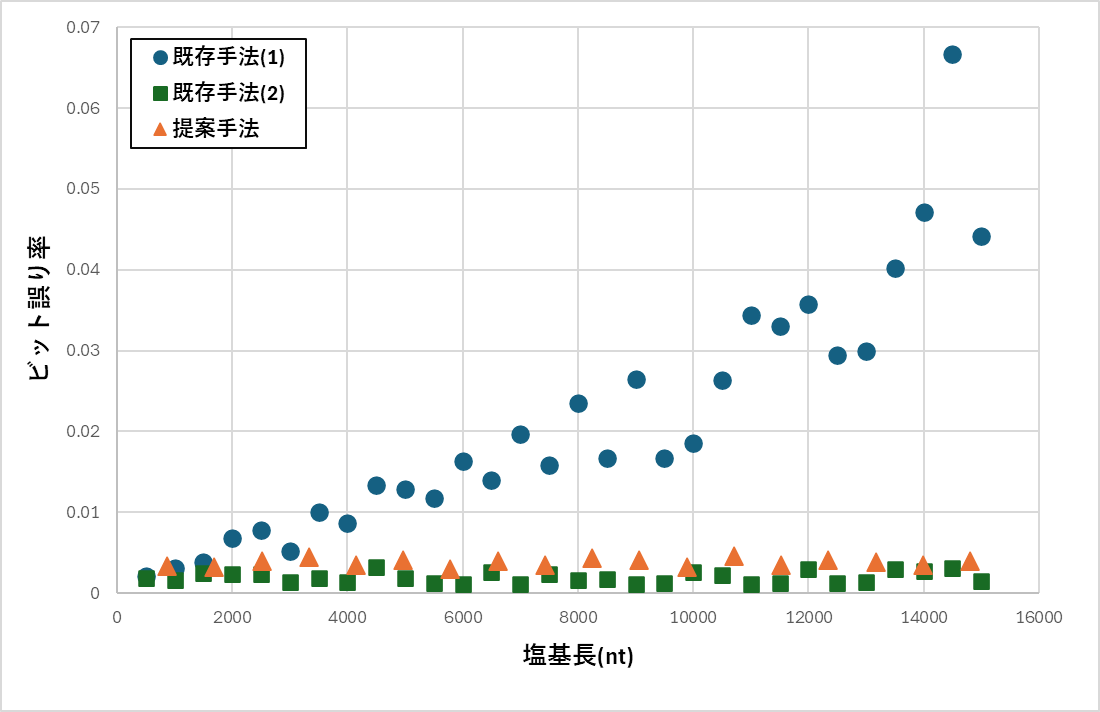
\includegraphics[width=120mm]{longread1.png}
  \caption{Relationship between base length and bit error rate}
  \label{fig:long_read_results1}
\end{figure}
\begin{figure}
  \centering
  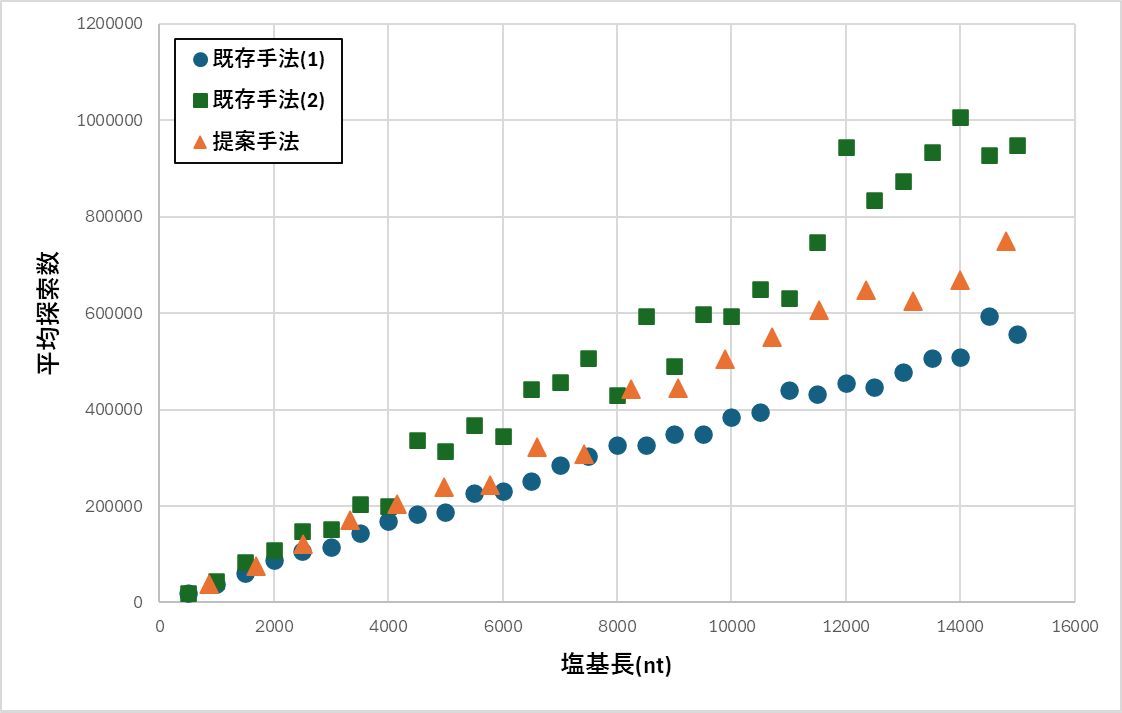
\includegraphics[width=120mm]{longread2.png}
  \caption{Relationship between base length and average number of heap searches per DNA strand}
  \label{fig:long_read_results2}
\end{figure}
\chapter{結論}
本研究では，DNAストレージの読み出しにおいてナノポアシーケンサーを用いることを前提とした
誤り訂正手法を提案し，その性能をシミュレーションにより評価した．
既存手法であるHEDGESは，DNAストレージにおけるシーケンス制約を満たしつつ
挿入・消失・置換エラーへの耐性を持つ誤り訂正符号であるが，
その復号アルゴリズムにおいて，
ナノポアシーケンサーでのDNA読み出しを前提とした最適化が行われていないという課題と，
DNA鎖の塩基長が長い場合に復号精度が低下するという課題が存在した．

本研究では，これらの課題を解決するために，
まずHEDGESの復号アルゴリズムにおいて，
ナノポアシーケンサーの統計的な読み出し特性とベースコーラーのCTC出力を
考慮した探索手法を提案した．
実験結果より，提案手法では既存手法と比較して復号アルゴリズムにおける探索数を
64\%から68\%削減し，
復号失敗によるビット消失率を76\%から83\%低減できることを示した．
さらに，ロングリードに向けた符号化・復号アルゴリズムの改良を提案し，
セグメント化による手法を用いることで長い塩基長のDNAを扱う場合の
復号精度の低下を抑制できることを示した．

今後の課題としては，以下の点が挙げられる．
第一に，ナノポアシーケンサーの出力特性をより詳細にモデル化することである．
本研究では，ラベル間の遷移確率のみを考慮した単純なモデルを用いたが，
塩基配列のコンテキスト依存性や，バースト的なエラー発生など，
より複雑な特性を考慮することで，復号における探索をより最適化できる可能性がある．
第二に，ベースコーラーの最新アーキテクチャに対応することである．
本研究で使用したBonitoはCNN-LSTM-CTC構成であるが，
最新のベースコーラーではCRFを用いたアーキテクチャなど，より先進的な機械学習手法が採用されており，
これらに対応することで復号精度のさらなる向上が期待できる．
第三に，実際のDNAを用いた実験的検証である．
本研究はシミュレーションのみによる評価であるため，
実際に合成DNAを用いたナノポアシーケンサーでの読み出し実験を行うことで，
提案手法の実用性を検証する必要がある．


%======================================================================
%		謝辞
%======================================================================
\begin{acknowledgements}
本研究を進めるにあたり，ご指導・ご助言を賜りました佐藤高史教授に
深く感謝申し上げます．
研究会やミーティングを通じて多くの貴重なご指摘・ご助言をいただきました
粟野皓光准教授，橋本昌宜教授，上野嶺准教授，白井僚助教，新津葵一教授，劉昆洋助教
に深く感謝致します．日々の研究において様々な助言をいただきました
小池健文氏に深く感謝いたします．
研究室生活において様々な面から支えて頂いた佐藤高史研究室支援職員の
西山修子氏，上西香織氏に感謝致します．
最後に，日頃から様々なご支援，ご協力を頂きました
佐藤研究室，橋本研究室，新津研究室の皆様に感謝致します．
\end{acknowledgements}



%======================================================================
%		参考文献
%======================================================================
\bibliographystyle{kueethesis}
\bibliography{reference}



%======================================================================
%		付録
%======================================================================
\appendix
\chapter{復号の探索効率化における予備実験}
\section{実験方法}
まず，ナノポアシーケンサーの出力特性を表す行列$\bm{P}_{\mathrm{STATS}}$を得るため，
ランダムなバイナリデータをHEDGESで符号化した複数のDNA鎖に対し，
ナノポアシーケンサーによる電流波形をSquigulatorを用いて
シミュレーションした．
次に，シミュレーションされた電流波形に対してBonitoを用いて
CTC出力を取得し，\ref{ctc_output}節で述べた方法で$\bm{P}_{\mathrm{CTC}}$を得た．
ここで，HEDGES符号化結果における$j$番目のDNA鎖の$i$番目の塩基を$C_i^{(j)}$と表し，
この塩基配列を$\{C_i^{(j)}\}$とする．また，
$\{C_i^{(j)}\}$のベースコールにおいて得られた
$\bm{P}_{\mathrm{CTC}}$を$\bm{P}_{\mathrm{CTC}}^{(j)}$と表すこととし，
$\bm{P}_{\mathrm{CTC}}^{(j)}$の各行において，出力確率が最大となる塩基を選択することで
得られる塩基配列を$\{C'^{(j)}_i\}$と表す．この$\{C'^{(j)}_i\}$と$\{C_i^{(j)}\}$に対して
グローバルアラインメントを行い，各塩基ごとに
正しい読み出し，置換・挿入・消失エラーの発生数を集計した\cite{GOTOH1982705}．
これを全ての$j$について行い，集計することで
各事象の発生確率を計算し，行列$\bm{P}_{\mathrm{STATS}}$を得た．

$\mu_{\mathrm{STATS}\_\mathrm{ok}}$，$\mu_{\mathrm{STATS}\_\mathrm{sub}}$，
$\mu_{\mathrm{STATS}\_\mathrm{ins}}$，$\mu_{\mathrm{STATS}\_\mathrm{del}}$はそれぞれ，正しい読み出し，置換エラー，
挿入エラー，消失エラーが発生したときの$\bm{P}_{\mathrm{STATS}}$のスコアの期待値であるから，
\begin{align}
  \mu_{\mathrm{STATS}\_\mathrm{ok}} &= \dfrac{\displaystyle \sum_{X \in \{A,C,G,T\}} p_{XX} \bm{P}_{\mathrm{STATS}}(X,X)}{\displaystyle \sum_{X \in \{A,C,G,T\}} p_{XX}} \\
  \mu_{\mathrm{STATS}\_\mathrm{sub}} &= \dfrac{\displaystyle \sum_{X,Y \in \{A,C,G,T\}, X \neq Y} p_{XY} \bm{P}_{\mathrm{STATS}}(X,Y)}{\displaystyle \sum_{X,Y \in \{A,C,G,T\}, X \neq Y} p_{XY}} \\
  \mu_{\mathrm{STATS}\_\mathrm{ins}} &= \dfrac{\displaystyle \sum_{Y \in \{A,C,G,T\}} p_{NY} \bm{P}_{\mathrm{STATS}}(N,Y)}{\displaystyle \sum_{Y \in \{A,C,G,T\}} p_{NY}} \\
  \mu_{\mathrm{STATS}\_\mathrm{del}} &= \dfrac{\displaystyle \sum_{X \in \{A,C,G,T\}} p_{XN} \bm{P}_{\mathrm{STATS}}(X,N)}{\displaystyle \sum_{X \in \{A,C,G,T\}} p_{XN}}
\end{align}
により計算される．
$\mu_{\mathrm{CTC}\_\mathrm{ok}}$，$\mu_{\mathrm{CTC}\_\mathrm{sub}}$，
$\mu_{\mathrm{CTC}\_\mathrm{ins}}$はそれぞれ，$\bm{P}_{\mathrm{CTC}}$において
正しい読み出し，置換エラー，挿入エラーに対応するスコアの期待値であるから，
\begin{align}
  \mu_{\mathrm{CTC}\_\mathrm{ok}} &= \dfrac{1}{M}\sum_j \sum_i \bm{P}_{\mathrm{CTC}}^{(j)}(i, C'^{(j)}_i) \\
  \mu_{\mathrm{CTC}\_\mathrm{sub}} &= \dfrac{1}{3M}\sum_j \sum_i \sum_{X \in \{A,C,G,T\}, X \neq C'^{(j)}_i} \bm{P}_{\mathrm{CTC}}^{(j)}(i, X) \\
  \mu_{\mathrm{CTC}\_\mathrm{ins}} &= \dfrac{1}{M}\sum_j \sum_i \bm{P}_{\mathrm{CTC}}^{(j)}(i, N)
\end{align}
により計算される．
ただし，$M$はベースコールされた全てのDNA鎖における塩基数の総和を表す．

次に，式\eqref{opt1}から\eqref{opt4}に示した
固定の報酬とペナルティ$P_{\mathrm{ok}}, P_{\mathrm{sub}}, P_{\mathrm{ins}}, P_{\mathrm{del}}$
及び各補正項の重み付けパラメータ
$\alpha_{\mathrm{ok}}, \alpha_{\mathrm{sub}}, \alpha_{\mathrm{ins}}, \alpha_{\mathrm{del}},
\beta_{\mathrm{ok}}, \beta_{\mathrm{sub}}, \beta_{\mathrm{ins}}$の最適な値を決定する．
ここで，$P_{\mathrm{ok}}$には文献\cite{HEDGES}用いられた値を各符号化率ごとに使用し，
$P_{\mathrm{ok}}$以外のパラメータを最適化した．
各パラメータの最適化は，復号におけるヒープの探索数を目的関数として
数値微分を用いた勾配降下法により行った．
具体的には，まずランダムに生成したバイナリデータをHEDGESで符号化し，
ナノポアシーケンサーでの読み出しをシミュレーションした上で
その電流波形に対してベースコーラーを適用し，CTC出力を得た．
勾配降下法によるパラメータの最適化は，このCTC出力の復号を対象として，
以下の手順で行った．
\begin{enumerate}
  \item 最適化対象の各パラメータを適当な初期値で初期化する．
  \item 提案手法を用いて復号を実施し，復号が完了するまでのヒープの探索数を計測する．
  \item 各パラメータごとに微小な値$\Delta$を加えた場合の復号における
  ヒープの探索数を計測する．
  \item これらの値を用いて各パラメータに関する目的関数の勾配を計算する．
  \item 各パラメータを学習率$\eta$を用いて以下のように更新する．
  \begin{align}
    \bm{\theta} \leftarrow \bm{\theta} - \eta \dfrac{\partial J}{\partial \bm{\theta}}
  \end{align}
  ここで，$\theta$は最適化対象の各パラメータを表し，$J$は目的関数を表す．
  \item 2から5を一定回数繰り返す．
\end{enumerate}
パラメータの最適化については，ナノポアシーケンサーの読み出し特性に基づく補正項と
CTC出力に基づく補正項の両方を用いる場合と，それぞれ一方のみを用いる場合について
効果を検証するため，
$P_{\mathrm{sub}}$,$P_{\mathrm{ins}}$,$P_{\mathrm{del}}$,$\alpha_{\mathrm{ok}}$, $\alpha_{\mathrm{sub}}$, $\alpha_{\mathrm{ins}}$, $\alpha_{\mathrm{del}}$,
$\beta_{\mathrm{ok}}$, $\beta_{\mathrm{sub}}$, $\beta_{\mathrm{ins}}$の10個のパラメータに対して行うのに加えて，
$\alpha_{\mathrm{ok}}=\alpha_{\mathrm{sub}}=\alpha_{\mathrm{ins}}=\alpha_{\mathrm{del}}=0$として他の6個のパラメータに対してのみ
行う場合と
$\beta_{\mathrm{ok}}=\beta_{\mathrm{sub}}=\beta_{\mathrm{ins}}=0$として他の7個のパラメータに対してのみ
行う場合についても実施した．
なお，これらの最適化は符号化率$0.75,0.60,0.50,0.33$について
それぞれ独立に行った．

\section{実験条件}
行列$\bm{P}_{\mathrm{STATS}}$を得るためのシミュレーションでは，ランダムに生成した400\,KBのバイナリデータを
HEDGESで符号化率を0.50として符号化した．各DNA鎖の塩基長は400\,ntとし，
合計12240本のDNA鎖を生成した．
Squigulatorによる電流値シミュレーションのパラメータ設定，
ベースコーラーのモデルについては\ref{sim1}節の実験と同様である．

ベースコーラーのファインチューニングには，
ランダムに生成した200\,KBのバイナリデータを
HEDGESで符号化率0.50，塩基長400\,ntで符号化して得られた6120本のDNA鎖と，
これらのDNA鎖に対してSquigulatorでシミュレーションした電流波形を学習データとして用いた．
既存の学習済みモデルである
dna\_r9.4.1@v2の重みを初期値として，バッチサイズを64として1エポックあたり75ステップ
の学習を行い，エポック数は50としてファインチューニングを行った．

$\{C^{(n)}_i\}$と$\{C'^{(n)}_i\}$に対するアラインメントにはBiopythonの
Gotohアルゴリズムを用いたグローバルアラインメントを使用した\cite{biopython,GOTOH1982705}．

パラメータの最適化では，ランダムに生成した400\,KBのバイナリデータを符号化率
$0.75,0.60,0.50,0.33$で塩基長を400\,ntとしてHEDGES符号化したものに対して
電流波形シミュレーションとベースコールを行って得られたCTC出力を用いた．
$P_{\mathrm{ok}}$は各符号化率ごとに表\ref{tab:fixed_reward}に示す固定値を使用した．
各パラメータの初期値は$P_{\mathrm{sub}}=P_{\mathrm{ins}}=P_{\mathrm{del}}=1.0$，
$\alpha_{\mathrm{ok}}=\alpha_{\mathrm{sub}}=\alpha_{\mathrm{ins}}=\alpha_{\mathrm{del}}=0.0$，
$\beta_{\mathrm{ok}}=\beta_{\mathrm{sub}}=\beta_{\mathrm{ins}}=0.0$とした．
学習率は符号化率ごとに表\ref{tab:learning_rate}に示す値を使用し，パラメータの更新を300回繰り返した．
\begin{table}
  \centering
  \begin{minipage}{0.48\linewidth}
    \centering
    \caption{符号化率ごとの報酬値$P_{\mathrm{ok}}$}
    \label{tab:fixed_reward}
    \begin{tabular}{c|c}
      \hline
      符号化率 & $P_{\mathrm{ok}}$ \\
      \hline
      0.75 & -0.035 \\
      0.60 & -0.082 \\
      0.50 & -0.127 \\
      0.33 & -0.229 \\
      \hline
    \end{tabular}
  \end{minipage}
  \hfill
  \begin{minipage}{0.48\linewidth}
    \centering
    \caption{符号化率ごとの学習率$\eta$}
    \label{tab:learning_rate}
    \begin{tabular}{c|c}
      \hline
      符号化率 & $\eta$ \\
      \hline
      0.75 & $1.3 \times 10^{-7}$ \\
      0.60 &  $4.1 \times 10^{-7}$\\
      0.50 &  $1.0 \times 10^{-6}$ \\
      0.33 &  $3.8 \times 10^{-6}$ \\
      \hline
    \end{tabular}
  \end{minipage}
\end{table}
なお，$\bm{P}_{\mathrm{STATS}}$を得るためのシミュレーション，
ベースコーラーのファインチューニング，
パラメータの最適化に用いたランダムなバイナリデータは全て独立に生成したものである．

\section{結果}
ナノポアシーケンサーの読み出し特性の評価により得られた
ラベル$\{N,A,C,G,T\}$間の遷移確率は表\ref{tab:transition_matrix}に
示す．
\begin{table}
  \centering
  \caption{ラベル間の遷移確率}
  \label{tab:transition_matrix}
  \begin{tabular}{c|ccccc}
    \hline
    入力$\backslash$出力 & N & A & C & G & T \\
    \hline
    N & $0.000$ & $3.11 \times 10^{-4}$ & $3.11 \times 10^{-4}$ & $3.18 \times 10^{-4}$ & $3.86 \times 10^{-4}$  \\
    A & $9.28 \times 10^{-4}$ & $0.232$ & $5.03 \times 10^{-4}$ & $1.01 \times 10^{-3}$ & $3.94 \times 10^{-5}$ \\
    C & $5.95 \times 10^{-4}$ & $3.10 \times 10^{-4}$ & $0.244$ & $3.56 \times 10^{-4}$ & $1.27 \times 10^{-4}$ \\
    G & $8.27 \times 10^{-4}$ & $9.00 \times 10^{-4}$ & $6.60 \times 10^{-4}$ & $0.269$ & $5.13 \times 10^{-5}$ \\
    T & $6.73 \times 10^{-4}$ & $4.36 \times 10^{-5}$ & $1.55 \times 10^{-4}$ & $5.85 \times 10^{-5}$ & $0.247$ \\
    \hline
  \end{tabular}
\end{table}
この結果では，正しい読み取りは全体のうち99.1\%を占めており，
置換エラーは0.421\%，挿入エラーは0.133\%，消失エラーは0.302\%であった．
また，置換エラーはA,G間とC,T間で発生しやすい傾向が見られ，
特に，最も確率の低いA,T間の
置換と比べてA,G間の置換は約23倍の確率で発生することが分かった．
塩基ごとの置換エラー発生率の偏りは，
プリン塩基(A,G)とピリミジン塩基(C,T)の化学構造
の類似性に起因すると考えられている\cite{10.1371/journal.pone.0257521}．
NからA,C,G,Tへの遷移で表わされる挿入エラーは，
各塩基に対して同程度の確率で発生していた．
A,C,G,TからNへの遷移で表わされる消失エラーは，
A,GにおいてC,Tよりも比較的高い確率で発生していた．
この結果から得られた行列$\bm{P}_{\mathrm{STATS}}$は
式\eqref{eq:appendix_P_STATS}のようになった．
各補正項の期待値は表\ref{tab:appendix_mu_values}に示す．
各符号化率ごとに最適化されたペナルティと補正項の重み付けパラメータは
表\ref{tab:appendix_params_p}および表\ref{tab:appendix_params_alpha_beta}に示す．
\begin{align}
  \bm{P}_{\mathrm{STATS}} =
  \begin{bmatrix}
    -1.20 & -0.650 & -0.650 & -0.643 & -0.613 \\
    -0.580 & 0.130 & -0.670 & -0.590 & -1.25 \\
    -0.620 & -0.650 & 0.110 & -0.640 & -1.09 \\
    -0.550 & -0.520 & -0.590 & 0.160 & -1.53 \\
    -0.590 & -1.53 & -1.09 & -1.25 & 0.120 \\
  \end{bmatrix} \label{eq:appendix_P_STATS}
\end{align}

\begin{table}
  \centering
  \caption{得られた各期待値}
  \label{tab:appendix_mu_values}
  \begin{tabular}{c|c}
    \hline
    パラメータ & 値 \\
    \hline
    $\mu_{\mathrm{STATS}\_\mathrm{ok}}$ & 1.38 \\
    $\mu_{\mathrm{STATS}\_\mathrm{sub}}$ & 7.52 \\
    $\mu_{\mathrm{STATS}\_\mathrm{ins}}$ & 8.01 \\
    $\mu_{\mathrm{STATS}\_\mathrm{del}}$ & 7.17 \\
    $\mu_{\mathrm{CTC}\_\mathrm{ok}}$ & 0.111 \\
    $\mu_{\mathrm{CTC}\_\mathrm{sub}}$ & 6.85 \\
    $\mu_{\mathrm{CTC}\_\mathrm{ins}}$ & 2.78 \\
    \hline
  \end{tabular}
\end{table}

\begin{table}
  \centering
  \caption{符号化率ごとに最適化したペナルティ}
  \label{tab:appendix_params_p}
  \footnotesize
  \begin{tabular}{c|c|ccc}
    \hline
    符号化率 & 手法 & $P_{\mathrm{sub}}$ & $P_{\mathrm{ins}}$ & $P_{\mathrm{del}}$ \\
    \hline
    \multirow{3}{*}{0.75} & STATSのみ$^{*}$ & 0.630 & 0.650 & 0.687 \\
    & CTCのみ$^{**}$ & 0.837 & 0.912 & 0.765 \\
    & STATS+CTC$^{***}$ & 0.875 & 0.911 & 0.778 \\
    \hline
    \multirow{3}{*}{0.60} & STATSのみ$^{*}$ & 0.883 & 0.965 & 0.995 \\
    & CTCのみ$^{**}$ & 0.856 & 1.06 & 0.890 \\
    & STATS+CTC$^{***}$ & 1.08 & 1.17 & 1.02 \\
    \hline
    \multirow{3}{*}{0.50} & STATSのみ$^{*}$ & 0.988 & 1.17 & 1.25 \\
    & CTCのみ$^{**}$ & 0.953 & 1.11 & 1.04 \\
    & STATS+CTC$^{***}$ & 1.15 & 1.23 & 1.19 \\
    \hline
    \multirow{3}{*}{0.33} & STATSのみ$^{*}$ & 1.07 & 1.25 & 1.39 \\
    & CTCのみ$^{**}$ & 1.06 & 1.22 & 1.21 \\
    & STATS+CTC$^{***}$ & 1.29 & 1.35 & 1.34 \\
    \hline
  \end{tabular}
  
  \small
  \vspace{0.3cm}
  
  \noindent
  \begin{tabular}{@{}l@{}}
    $^{*}$STATSのみ: ナノポアシーケンサーの読み出し特性に基づく補正項のみを使用 \\
    $^{**}$CTCのみ: CTC出力に基づく補正項のみを使用 \\
    $^{***}$STATS+CTC: ナノポアシーケンサーの読み出し特性およびCTC出力の両方に基づく補正項を使用
  \end{tabular}
\end{table}

\begin{table}
  \centering
  \caption{符号化率ごとに最適化した補正項の重み付けパラメータ}
  \label{tab:appendix_params_alpha_beta}
  \footnotesize
  \begin{tabular}{c|c|cccc|ccc}
    \hline
    符号化率 & 手法 & $\alpha_{\mathrm{ok}}$ & $\alpha_{\mathrm{sub}}$ & $\alpha_{\mathrm{del}}$ & $\alpha_{\mathrm{ins}}$ & $\beta_{\mathrm{ok}}$ & $\beta_{\mathrm{sub}}$ & $\beta_{\mathrm{ins}}$ \\
    \hline
    \multirow{3}{*}{0.75} & STATSのみ& 0.0605 & 0.116 & 0.0929 & 0.0952 & 0.00 & 0.00 & 0.00 \\
    & CTCのみ& 0.00 & 0.00 & 0.00 & 0.00 & -0.192 & 0.211 & 0.347 \\
    & STATS+CTC& 0.00668 & 0.130 & -0.0105 & 0.544 & -0.150 & 0.181 & 0.301 \\
    \hline
    \multirow{3}{*}{0.60} & STATSのみ & 0.00513 & 0.256 & 0.200 & 0.0969 & 0.00 & 0.00 & 0.00 \\
    & CTCのみ & 0.00 & 0.00 & 0.00 & 0.00 & -0.223 & 0.190 & 0.419 \\
    & STATS+CTC & 0.110 & 0.243 & 0.236 & 0.219 & -0.115 & 0.184 & 0.330 \\
    \hline
    \multirow{3}{*}{0.50} & STATSのみ & 0.0548 & 0.294 & 0.0800 & 0.0871 & 0.00 & 0.00 & 0.00 \\
    & CTCのみ & 0.00 & 0.00 & 0.00 & 0.00 & -0.108 & 0.193 & 0.411 \\
    & STATS+CTC & 0.131 & 0.292 & 0.234 & 0.176 & -0.136 & 0.188 & 0.467 \\
    \hline
    \multirow{3}{*}{0.33} & STATSのみ & -0.00773 & 0.282 & 0.167 & 0.246 & 0.00 & 0.00 & 0.00 \\
    & CTCのみ & 0.00 & 0.00 & 0.00 & 0.00 & 0.0272 & 0.145 & 0.422 \\
    & STATS+CTC & 0.0260 & 0.328 & 0.177 & 0.230 & 0.0417 & 0.134 & 0.460 \\
    \hline
  \end{tabular}
\end{table}


\end{document}
% Local Variables:
% fill-column: 70
% End:
